\RequirePackage{silence}
\WarningFilter{babel}{Name 'brazil' is deprecated}
\WarningFilter{memoir}{\settocpreprocessor is marked deprecated}

\documentclass[
	% -- opções da classe memoir --
	12pt,				% tamanho da fonte
	openright,			% capítulos começam em pág ímpar (insere página vazia caso preciso)
	oneside,			% para impressão em frente e verso. Oposto a oneside
	a4paper,			% tamanho do papel.
	% -- opções da classe abntex2 --
	chapter=TITLE,		% títulos de capítulos convertidos em letras maiúsculas
	section=TITLE,		% títulos de seções convertidos em letras maiúsculas
	subsection=TITLE,	% títulos de subseções convertidos em letras maiúsculas
	subsubsection=TITLE,% títulos de subsubseções convertidos em letras maiúsculas
	% -- opções do pacote babel --
	english,			% idioma adicional para hifenização
	brazilian			% o último idioma é o principal do documento
	]{abntex2}



% ---
% Pacotes básicos 
% ---
%\usepackage{lmodern}			% Usa a fonte Latin Modern
\usepackage{mathptmx}			% Usa a fonte Times New Roman
%\usepackage{helvet}			% Fonte Parecida com Arial
\usepackage[T1]{fontenc}		% Selecao de codigos de fonte.
\usepackage[utf8]{inputenc}		% Codificacao do documento (conversão automática dos acentos)
\usepackage{lastpage}			% Usado pela Ficha catalográfica
\usepackage{indentfirst}			% Indenta o primeiro parágrafo de cada seção.
\usepackage{color}				% Controle das cores
\usepackage{graphicx}			% Inclusão de gráficos
\usepackage{subcaption}			% Inclusão de gráficos lado a lado
\usepackage{microtype} 			% para melhorias de justificação
\usepackage{tabularx,ragged2e}	% Para inserir tabelas
\usepackage{multirow}			% Para mesclar células
\usepackage[dvipsnames,table,xcdraw]{xcolor}		% Permite adicionar cores nas linhas de tabelas
\usepackage{fancyvrb}			% Permite adicionar arquivos de texto
\usepackage[portuguese, ruled, linesnumbered]{algorithm2e} % Uso de algoritmos
\usepackage{amsfonts}			% Permite usar notação de conjuntos
\usepackage{amsmath}			% Permite citar equações
\usepackage{amsthm}				% Permite criar teoremas e experimentos
\usepackage[font={bf, small}, labelsep=endash, labelfont=bf]{caption}	% Faz legenda de figuras ficarem em negrito
\usepackage{cancel}				% Permite fazer expressão tendendo a zero
\usepackage{epstopdf}			% Converte eps para pdf
\usepackage[final]{pdfpages}
\usepackage{hyphenat}
\usepackage{longtable}
\usepackage{graphicx}
\usepackage[section]{placeins}

\usepackage{tikz}
\usepackage{xcolor}
\usepackage{amsmath}
\usetikzlibrary{positioning, arrows.meta, shapes.geometric}
\newcolumntype{L}{>{\RaggedRight\arraybackslash}X}
% ---
		
% ---
% Pacotes adicionais, usados apenas no âmbito do Modelo Canônico do abnteX2
% ---
\usepackage{lipsum}				% para geração de dummy text
% ---
\usepackage{xcolor}
% ---
% Pacotes de citações
% ---
%\usepackage[brazilian,hyperpageref]{backref}	 % Paginas com as citações na bibl
\usepackage[alf, abnt-emphasize=bf]{abntex2cite}	% Citações padrão ABNT

% ---
% Customizações para o layout da UFPA
% ---
\usepackage{modelo-ufpa/ufpa}

\tolerance=1
\emergencystretch=\maxdimen
\hyphenpenalty=10000
\hbadness=10000
\hyphenchar\font=-1
\sloppy
\renewcommand{\ABNTEXchapterfontsize}{\normalsize}
\renewcommand{\ABNTEXsectionfontsize}{\normalsize}
\renewcommand{\ABNTEXsubsectionfontsize}{\normalsize}
\renewcommand{\ABNTEXsectionfont}{}
\renewcommand{\ABNTEXsubsectionfont}{}

\renewcommand{\chaptername}{ }
%\renewcommand{\familydefault}{\sfdefault} % usar apenas se usar a fonte helvet

% Muda o título de lista de ilustrações para lista de figuras
\addto\captionsbrazilian{%
  \renewcommand{\listfigurename}%
    {Lista de Ilustrações}%
	\renewcommand{\listtablename}%
    {Lista de Tabelas}%
}

% Permite utilizar figuras sem precisar colocar o caminho absoluto
\graphicspath{{imagens/}}

% Define o ambiente de experimentos
\theoremstyle{definition}
\newtheorem{experimento}{Experimento}[section]
\newcommand{\experimentoautorefname}{Experimento}

% --- 
% CONFIGURAÇÕES DE PACOTES
% --- 

% ---
% Configurações do pacote backref
% Usado sem a opção hyperpageref de backref
%\renewcommand{\backrefpagesname}{Citado na(s) página(s):~}
% Texto padrão antes do número das páginas
%\renewcommand{\backref}{}
% Define os textos da citação
%\renewcommand*{\backrefalt}[4]{
%	\ifcase #1 %
%		Nenhuma citação no texto.%
%	\or
%		Citado na página #2.%
%	\else
%		Citado #1 vezes nas páginas #2.%
%	\fi}%
% ---

% ---
% Informações de dados para CAPA, FOLHA DE ROSTO e FICHA CATALOGRÁFICA
% ---
\universidade{CENTRO UNIVERSITÁRIO SERRA DOS ÓRGÃOS - UNIFESO}
\instituto{DIREÇÃO ACADÊMICA DE CIÊNCIAS HUMANAS E TECNOLÓGICAS - DACHT}
\curso{CURSO DE BACHARELADO EM CIÊNCIA DA COMPUTAÇÃO}
\titulo{Detecção de Anomalias e Análise Probabilística em Manobras de Energização de Linhas de Transmissão Utilizando Aprendizagem de Máquina}
\autor{Kleber Daniel Mattos Viana}
\local{TERESÓPOLIS}
\data{2026}
\orientador{Prof. Andressa Alves Machado da Silva}
\coorientador{Prof. Bráulio Chuco Paucar} %CASO HAJA UM
\tipotrabalho{Monografia}
\preambulo{Trabalho de Conclusão de Curso apresentado ao Centro Universitário Serra dos Órgãos como requisito obrigatório para obtenção do título de Bacharel em Ciência da Computação.}
\sobrenome{Mattos Viana}
\nome{Kleber Daniel}% APENAS O PRIMEIRO NOME SEM SOBRENOME
\palavraschave{%
Sobretensões transitórias,
Detecção de anomalias,
Aprendizagem de máquina,
ATP/EMTP,
Análise probabilística.
}

\datadadefesa{Data da Defesa: 28 de Novembro de 2026}% PREENCHER COM O DATA DA DEFESA}
%\conceito{Conceito: Excelente}
\faculdadedoorientador{Centro Universitário Serra dos Órgãos} %
\titulacaodoorientador{DSc}%Coloque abreviado a titulação do seu Orientador
\faculdadedocoorientador{Centro Universitário Serra dos Órgãos}
\titulacaodocoorientador{DSc.}
\primeiromembrodabanca{A definir}
\titulacaodoprimeiromembro{DSc}
\faculdadedoprimeiromembrodabanca{A definir}
\segundomembrodabanca{A definir}
\titulacaodosegundomembro{DSc}
\faculdadedosegundomembrodabanca{A definir}
% ---

% ---
% Configurações de aparência do PDF final

% alterando o aspecto da cor azul
\definecolor{blue}{RGB}{41,5,195}

% informações do PDF

\makeatletter
\hypersetup{
     	%pagebackref=true,
		pdftitle={\imprimirtitulo}, 
		pdfauthor={\imprimirautor},
    	pdfsubject={\imprimirpreambulo},
	    pdfcreator={LaTeX with abnTeX2},
		pdfkeywords={\imprimirpalavraschave}, 
		colorlinks=true,       		% false: boxed links; true: colored links
    	linkcolor=black,          	% color of internal links
    	citecolor=black,        		% color of links to bibliography
    	filecolor=magenta,      		% color of file links
		urlcolor=black,
		bookmarksdepth=4,
        breaklinks=true
}
\makeatother


% --- 

% --- 
% Espaçamentos entre linhas e parágrafos 
% --- 

% O tamanho do parágrafo é dado por:
\setlength{\parindent}{1.5cm}

% Controle do espaçamento entre um parágrafo e outro:
\setlength{\parskip}{0.2cm}  % tente também \onelineskip

% ---
% compila o indice
% ---
\makeindex
% ---

% ----
% Início do documento
% ----
\begin{document}

\hypersetup{pageanchor=false}

% Seleciona o idioma do documento (conforme pacotes do babel)
%\selectlanguage{english}
\selectlanguage{brazilian}

% Retira espaço extra obsoleto entre as frases.
\frenchspacing 


% ----------------------------------------------------------
% ELEMENTOS PRÉ-TEXTUAIS
% ----------------------------------------------------------
% \pretextual

% ---
% Capa
% ---
\imprimircapa
% ---

% ---
% Folha de rosto
% ---
\imprimirfolhaderosto
% ---

% ---
% Inserir a ficha bibliografica
% ---
% A biblioteca da universidade lhe fornecerá um PDF
% com a ficha catalográfica definitiva após a defesa do trabalho. Quando estiver
% com o documento, salve-o como PDF no diretório do seu projeto e substitua todo
% o conteúdo de implementação deste arquivo pelo comando abaixo:

%\begin{fichacatalografica}
%    \includepdf{fichacatalografica.pdf}
%\end{fichacatalografica}


\newpage
% ---
% ---

% ---
% Inserir folha de aprovação
% ---
%
\begin{folhadeaprovacao}
\imprimirfolhadeaprovacao
\end{folhadeaprovacao}


% ---

% ---
% Dedicatória
% ---

% ESCREVA A SUA DEDICATORIA A DEDICATORIA QUE SE ENCONTRA NO ARQUIVO E APENAS UM EXEMPLO. ESCOLHA A DEDICATORIA QUE MAIS LHE AGRADAR. LEMBRE-SE DE UTILIZAR AS '\\' PARA PULAR LINHAS

\begin{dedicatoria}
   \vspace*{\fill}
   \flushright
   %\noindent
   \textit{Este trabalho é dedicado às crianças adultas que,\\
   quando pequenas, sonharam em se tornar cientistas. \\
   - Lauro César}
\end{dedicatoria}
% ---

% ---
% Agradecimentos
% ---
\begin{agradecimentos}

Agradeço à minha orientadora, Prof. Andressa Alves Machado da Silva, e ao meu coorientador, Prof. Bráulio Chuco Paucar, pelo apoio, pela orientação e pelas contribuições ao desenvolvimento deste trabalho. Agradeço também aos professores do curso de Bacharelado em Ciência da Computação do Centro Universitário Serra dos Órgãos, aos colegas que contribuíram ao longo da formação acadêmica e à minha família pelo incentivo durante esta trajetória.

\end{agradecimentos}
% ---

% ---
% Epígrafe
% ---

% ESCREVA A SUA EPÍGRAFE A MESMA QUE SE ENCONTRA NO ARQUIVO E APENAS UM EXEMPLO. ESCOLHA A EPÍGRAFE QUE MAIS LHE AGRADAR. LEMBRE-SE DE UTILIZAR AS '\\' PARA PULAR LINHAS

\begin{epigrafe}
    \vspace*{\fill}
	\begin{flushright}
		\textit{``Ciência é o que entendemos bem o suficiente para explicar a um computador.\\ 
		Arte é tudo o mais que fazemos.'' \\ 
		(Donald Knuth)}
	\end{flushright}
\end{epigrafe}
% ---

% ---
% RESUMOS
% ---


% ---

% ---
% inserir lista de ilustrações
% ---
% UTILIZE CASO HAJA FIGURAS NA MONOGRAFIAS. EM QUASO DE AUSENCIA DE FIGURAS COMENTAR COM AS 3 LINHAS DE CODIGOS UTILIZANDO O '%'.
\pdfbookmark[0]{\listfigurename}{lof}
\listoffigures*
\cleardoublepage
% ---

% ---
% inserir lista de quadros
% ---
% UTILIZE CASO HAJA QUADROS NA MONOGRAFIAS. EM QUASO DE AUSENCIA DE QUADROS COMENTAR COM AS 3 LINHAS DE CODIGOS UTILIZANDO O '%'.

% \pdfbookmark[0]{\listofquadrosname}{loq}
% \listofquadros*
% \cleardoublepage
% ---

% ---
% inserir lista de tabelas
% ---

% UTILIZE QUASE HAJA TABELAS NA MONOGRAFIAS. EM QUASO DE AUSENCIA DE TABELAS COMENTAR COM AS 3 LINHAS DE CODIGOS UTILIZANDO O '%'.

% \pdfbookmark[0]{\listtablename}{lot}
% \listoftables*
% \cleardoublepage
% ---

% ---
% inserir lista de algoritmos
% ---

% UTILIZE CASO HAJA ALGORITMOS NA MONOGRAFIAS. EM QUASO DE AUSENCIA DE ALGORITMOS COMENTAR COM AS 3 LINHAS DE CODIGOS UTILIZANDO O '%'.

% \pdfbookmark[0]{\listalgorithmcfname}{loa}
% \imprimirlistadealgoritmos
% \cleardoublepage
% ---

% ---
% inserir lista de abreviaturas e siglas
% ---
% DEVE SER PREENCHIDA A MÃO LEMBRE-SE DE MANTER EM ORDEM ALFABETICA.
\begin{siglas}
  \item[ABNT] Associação Brasileira de Normas Técnicas
  \item[ANAFAS] Programa de Análise de Faltas Simultâneas
  \item[ANAREDE] Programa de Análise de Redes Elétricas
  \item[ATP] \textit{Alternative Transients Program}
  \item[ATPDraw] Interface gráfica para elaboração de modelos do ATP
  \item[DBSCAN] \textit{Density-Based Spatial Clustering of Applications with Noise}
  \item[EMTP] \textit{Electromagnetic Transients Program}
  \item[IA] Inteligência Artificial
  \item[LT] Linha de transmissão
  \item[ONS] Operador Nacional do Sistema Elétrico
  \item[PAR/PEL] Plano da Operação Elétrica de Médio Prazo
\end{siglas}
% ---

% ---
% inserir lista de símbolos
% ---
% DEVE SER PREENCHIDA A MÃO LEMBRE-SE DE MANTER EM ORDEM ALFABETICA.
\begin{simbolos}
  \item[$\varepsilon$] Raio de vizinhança utilizado pelo algoritmo DBSCAN
  \item[$k$] Número de agrupamentos utilizado pelo algoritmo K-Means
  \item[$\mu$] Média do conjunto de dados analisado
  \item[$\sigma$] Desvio padrão do conjunto de dados analisado
  \item[$N$] Número total de observações ou simulações consideradas
\end{simbolos}
% ---

% resumo em português
\setlength{\absparsep}{18pt} % ajusta o espaçamento dos parágrafos do resumo
\begin{resumo}

Este trabalho apresenta uma proposta computacional para automatizar a extração, o tratamento estatístico, a análise probabilística e a classificação de dados provenientes de simulações de transitórios eletromagnéticos em manobras de energização de linhas de transmissão. O estudo parte do problema de que a inspeção manual dos arquivos gerados pelo \textit{Alternative Transients Program} (ATP) pode ser lenta, repetitiva e suscetível a interpretações inconsistentes, especialmente quando há múltiplas simulações e grande volume de resultados. A proposta considera a identificação de sobretensões máximas, a caracterização estatística dos dados, o uso de critérios preliminares para detecção de valores extremos e a aplicação de técnicas de aprendizagem de máquina não supervisionada, como K-Means e DBSCAN, para auxiliar na identificação de padrões de comportamento e possíveis anomalias. Espera-se que a integração entre análise estatística, visualização de dados e algoritmos de clusterização contribua para reduzir a subjetividade da avaliação técnica e oferecer suporte mais consistente à interpretação dos resultados de simulações de energização.

 \textbf{Palavras-chave}: \imprimirpalavraschave
\end{resumo}

% resumo em inglês
\begin{resumo}[Abstract]
 \begin{otherlanguage*}{english}
   This work presents a computational proposal to automate the extraction, statistical treatment, probabilistic analysis and classification of data obtained from electromagnetic transient simulations in transmission line energization maneuvers. The study addresses the problem that the manual inspection of files generated by the \textit{Alternative Transients Program} (ATP) can be slow, repetitive and susceptible to inconsistent interpretations, especially when multiple simulations and large volumes of results are involved. The proposed approach considers the identification of maximum overvoltages, the statistical characterization of data, the use of preliminary criteria for extreme-value detection and the application of unsupervised machine learning techniques, such as K-Means and DBSCAN, to support the identification of behavioral patterns and possible anomalies. The integration of statistical analysis, data visualization and clustering algorithms is expected to reduce the subjectivity of technical assessment and provide more consistent support for interpreting energization simulation results.

   \vspace{\onelineskip}
 
   \noindent 
   \textbf{Keywords}: Transient overvoltages. Anomaly detection. Machine learning. ATP/EMTP. Probabilistic analysis.
 \end{otherlanguage*}
\end{resumo}

% ---
% inserir o sumario
% ---
\pdfbookmark[0]{\contentsname}{toc}
\tableofcontents*
\cleardoublepage
% ---



% ----------------------------------------------------------
% ELEMENTOS TEXTUAIS
% ----------------------------------------------------------
\hypersetup{pageanchor=true}
\textual
\pagestyle{simple}

% ----------------------------------------------------------
% Introdução
% ----------------------------------------------------------
\chapter{Introdução}

A operação de sistemas elétricos de potência exige elevado grau de confiabilidade, especialmente em processos de energização de linhas de transmissão, nos quais podem surgir sobretensões transitórias capazes de comprometer a coordenação de isolamento dos equipamentos. 
Em sistemas de transmissão em alta tensão, os fenômenos transitórios associados às manobras de energização e religamento apresentam curta duração, porém podem atingir amplitudes significativas, influenciando diretamente a definição dos níveis de isolamento, a especificação de equipamentos e os critérios de segurança operacional \cite{iec6007112019,iec6007122023,marin2025}.

Nesse contexto, ferramentas de simulação eletromagnética são amplamente empregadas para antecipar comportamentos do sistema e subsidiar decisões de projeto. Entre essas ferramentas, o \textit{Alternative Transients Program/Electromagnetic Transients Program} (ATP/EMTP) se destaca por permitir a modelagem de transitórios eletromagnéticos em linhas de transmissão, considerando fenômenos dependentes da frequência e diferentes condições de manobra \cite{dommel1969,marti1982}.
A utilização de simulações computacionais é particularmente relevante nesse tipo de estudo, uma vez que os valores de sobretensão podem depender de fatores como o instante de fechamento dos polos do disjuntor, a configuração física da rede, os parâmetros elétricos da linha, a distância entre circuitos paralelos e as condições iniciais do sistema \cite{mestas2010,marin2025}.

% Apesar de sua relevância técnica, a análise dos resultados gerados pelo ATP ainda apresenta dificuldades importantes. Os arquivos de saída podem conter grande quantidade de informações, o que torna a inspeção manual lenta, repetitiva e suscetível a interpretações inconsistentes.
% Esse problema torna-se mais evidente em estudos com múltiplas simulações, especialmente quando são avaliadas diferentes condições de manobra, instantes de fechamento dos disjuntores ou configurações do sistema. Nesses casos, a avaliação dos resultados não deve se limitar apenas à identificação dos maiores valores de tensão, mas também considerar a distribuição dos dados, a frequência de ocorrência dos eventos críticos e a coerência desses valores com o comportamento físico esperado do sistema.
% Além disso, nem todo valor extremo observado em uma simulação representa, necessariamente, a condição mais adequada para orientar uma decisão de projeto. Em alguns casos, picos isolados podem estar associados a condições operacionais muito específicas, comportamentos transitórios pouco representativos do conjunto analisado ou, ainda, a efeitos numéricos que precisam ser verificados por meio de uma análise mais criteriosa. Essa distinção é essencial, pois impacta diretamente a avaliação do nível de isolamento e, consequentemente, os custos e a segurança de projetos em sistemas de transmissão.
% Assim, a adoção direta do maior valor observado como única referência de projeto pode conduzir a interpretações excessivamente conservadoras, sobretudo quando esse valor corresponde a uma ocorrência isolada ou estatisticamente discrepante em relação ao conjunto de dados analisado. Por isso, torna-se importante combinar a análise dos valores máximos com critérios estatísticos e com a interpretação física do fenômeno transitório estudado.

Apesar da importância do ATP em estudos de transitórios eletromagnéticos, a análise dos arquivos gerados pelo programa ainda pode ser trabalhosa. Em simulações com muitos cenários, os resultados ficam distribuídos em arquivos extensos, exigindo que o usuário localize manualmente os maiores valores de sobretensão e organize essas informações para posterior interpretação. Esse processo, além de repetitivo, pode gerar inconsistências, principalmente quando diferentes instantes de fechamento dos disjuntores, fases e pontos de monitoramento são considerados. Por esse motivo, este trabalho propõe uma rotina computacional para auxiliar a análise dos resultados de energização de linhas de transmissão. A proposta não busca substituir a interpretação técnica do fenômeno elétrico, mas oferecer uma forma mais organizada e reprodutível de identificar valores máximos, observar padrões estatísticos e apontar possíveis anomalias no conjunto de simulações.

\section{Problema de pesquisa}

Diante desse cenário, este trabalho aborda o problema de como identificar, de forma mais confiável e automatizada, quais sobretensões máximas observadas em manobras de energização correspondem a eventos fisicamente relevantes e quais devem ser analisadas como possíveis anomalias ou \textit{outliers}. Assim, a questão central da pesquisa pode ser sintetizada da seguinte forma: de que maneira técnicas de tratamento estatístico, análise probabilística e aprendizagem de máquina não supervisionada podem auxiliar na diferenciação entre sobretensões coerentes com o fenômeno físico simulado e valores discrepantes presentes em bases produzidas por simulações estatísticas no ATP?

A detecção de anomalias em bases de dados de sistemas elétricos tem sido amplamente investigada com o apoio de técnicas estatísticas e algoritmos de aprendizagem de máquina, especialmente em aplicações relacionadas ao monitoramento de redes, identificação de falhas, análise de medições, detecção de ataques à integridade dos dados e reconhecimento de comportamentos incomuns em sistemas elétricos e \textit{smart grids} \cite{chandola2009,guato2024,ardebili2024,gillioz2026}. Embora esses estudos não estejam necessariamente voltados à análise de sobretensões transitórias geradas por simulações no ATP, eles fornecem base conceitual e metodológica para o uso de técnicas de detecção de anomalias na interpretação automatizada de dados provenientes de sistemas elétricos. Nesse contexto, métodos não supervisionados apresentam potencial de aplicação, pois permitem reconhecer estruturas internas nos dados e identificar observações discrepantes sem a necessidade de rotulação prévia das amostras \cite{guato2024,gillioz2026}.

\section{Justificativa}

A justificativa deste trabalho está relacionada à necessidade de tornar a análise de resultados de simulações de energização mais reprodutível, objetiva e tecnicamente consistente. Em estudos com grande quantidade de cenários, a inspeção manual dos arquivos de saída do ATP tende a aumentar o tempo de análise e a possibilidade de erros na organização dos dados. Além disso, a utilização direta do maior valor observado como única referência pode conduzir a interpretações excessivamente conservadoras quando esse valor corresponde a uma ocorrência isolada ou pouco representativa do conjunto analisado.

Parte-se da expectativa de que a combinação entre métodos estatísticos clássicos, análise probabilística e técnicas de aprendizagem de máquina não supervisionada contribua para tornar a avaliação mais robusta, reduzindo a subjetividade da inspeção manual e oferecendo suporte mais consistente à tomada de decisão em estudos de coordenação de isolamento. Algoritmos como K-Means e DBSCAN podem auxiliar, respectivamente, na identificação de agrupamentos predominantes e de regiões de baixa densidade associadas a observações atípicas \cite{ardebili2024}. Assim, além de contribuir para a confiabilidade técnica do processo analítico, a proposta pode favorecer a otimização de investimentos, ao evitar superdimensionamentos motivados por eventos sem relevância prática.

A proposta deste trabalho consiste, portanto, em desenvolver uma rotina computacional em Python capaz de integrar a extração, a organização, o tratamento estatístico, a análise probabilística e a classificação dos dados obtidos no ATP, oferecendo apoio à interpretação técnica das sobretensões máximas observadas em manobras de energização de linhas de transmissão.


\section{Objetivos}

\subsection{Objetivo geral}


Desenvolver um modelo computacional para automatizar a extração, o tratamento estatístico, a análise probabilística e a classificação de dados provenientes de simulações computacionais e estatísticas realizadas no \textit{Alternative Transients Program} (ATP), com foco na identificação de anomalias e valores extremos em manobras de energização de linhas de transmissão.


\subsection{Objetivos específicos}


Para alcançar o objetivo geral, são definidos os seguintes objetivos específicos:


\begin{itemize}
\item Implementar um \textit{parser} computacional para extração automática dos dados brutos presentes nos arquivos estatísticos gerados pelo ATP.


\item Organizar e estruturar os dados extraídos em formato adequado para análise computacional, possibilitando o tratamento das informações referentes às sobretensões máximas observadas nas fases do sistema.

\item Aplicar técnicas de pré-processamento e tratamento estatístico dos dados, incluindo cálculo de média, desvio padrão, medidas de dispersão e critérios baseados na regra empírica de $3\sigma$ para identificação preliminar de valores extremos.

\item Realizar análise probabilística das sobretensões máximas obtidas nas simulações, estimando níveis de confiança, frequências empíricas e probabilidades de ocorrência associadas a eventos extremos.

\item Aplicar algoritmos de aprendizagem de máquina não supervisionada, como K-Means e DBSCAN, para identificar agrupamentos de comportamento e detectar observações atípicas no conjunto de dados.

\item Comparar os resultados obtidos pelas técnicas estatísticas e pelos algoritmos de clusterização, avaliando a coerência das anomalias identificadas em relação ao comportamento global da base de dados.

\item Desenvolver uma rotina computacional reprodutível que integre as etapas de extração, tratamento, análise estatística, análise probabilística, detecção de anomalias e apresentação dos resultados.


\end{itemize}

\section{Organização do trabalho}

Este trabalho está organizado em capítulos que contemplam os principais elementos da investigação. Após esta introdução, o capítulo de fundamentação teórica apresenta os conceitos necessários para compreender o problema, incluindo aspectos de transitórios eletromagnéticos, simulação computacional, análise estatística, análise probabilística e técnicas de aprendizagem de máquina aplicadas à detecção de anomalias. O capítulo seguinte descreve a modelagem do sistema elétrico utilizada como ambiente de geração dos dados. Na sequência, o capítulo de metodologia e desenvolvimento apresenta os procedimentos de extração, tratamento e análise dos resultados, bem como a construção da solução proposta. Por fim, o capítulo de conclusão retoma os objetivos do estudo, sintetiza os resultados alcançados e aponta possibilidades de continuidade da pesquisa.

\chapter{Fundamentação teórica}

Este capítulo apresenta os principais conceitos necessários para a compreensão da proposta deste trabalho, relacionando o fenômeno físico investigado, os procedimentos computacionais utilizados para sua simulação e os métodos estatísticos e de aprendizagem de máquina empregados na análise dos resultados. A fundamentação teórica parte da operação de sistemas elétricos de potência e da ocorrência de sobretensões transitórias em linhas de transmissão, avançando para a simulação computacional com o \textit{Alternative Transients Program} (ATP), o tratamento estatístico dos dados, a visualização dos resultados, a detecção de anomalias e o uso de técnicas de aprendizagem de máquina não supervisionada. Essa organização permite compreender como os dados gerados por múltiplas simulações de energização podem ser analisados de forma automatizada, com o objetivo de apoiar a identificação de valores extremos, padrões de comportamento e possíveis anomalias.

% \section{Sistemas elétricos de potência e linhas de transmissão}

\section{Sistemas elétricos, linhas de transmissão e transitórios de energização}
Os sistemas elétricos de potência são responsáveis pela geração, transmissão, distribuição e utilização da energia elétrica. Nesse contexto, as linhas de transmissão desempenham papel fundamental, pois permitem o transporte de grandes blocos de energia entre centros geradores e centros consumidores. Por operarem normalmente em níveis elevados de tensão, essas linhas exigem planejamento cuidadoso, critérios adequados de proteção e avaliação constante de fenômenos capazes de comprometer a confiabilidade operacional do sistema. Durante a operação de uma linha de transmissão, diferentes eventos podem alterar temporariamente o comportamento das tensões e correntes, como abertura e fechamento de disjuntores, ocorrência de faltas, religamentos e energizações. Entre essas situações, as manobras de energização merecem destaque, pois podem produzir sobretensões transitórias superiores aos valores observados em regime permanente, influenciando diretamente a coordenação de isolamento dos equipamentos. Marin et al. \cite{marin2025} destacam que a análise de sobretensões transitórias em linhas de transmissão é essencial para a operação segura de sistemas de alta tensão, especialmente porque esses fenômenos podem atingir amplitudes significativas e afetar os critérios de isolamento e segurança operacional. Assim, valores superestimados podem conduzir ao aumento desnecessário dos custos de projeto, enquanto valores subestimados podem comprometer a segurança operacional e a vida útil dos componentes. Dessa forma, a análise adequada das sobretensões transitórias é essencial para conciliar confiabilidade técnica e viabilidade econômica em sistemas de transmissão.

% \section{Transitórios eletromagnéticos em manobras de energização}

Nesse sentido, compreender a natureza dos transitórios eletromagnéticos torna-se fundamental para avaliar adequadamente os efeitos das manobras de energização sobre o sistema. Transitórios eletromagnéticos são fenômenos de curta duração que ocorrem quando há uma alteração repentina nas condições elétricas de um sistema. Essas alterações podem ser provocadas por chaveamentos, descargas atmosféricas, faltas, rejeição de carga ou energização de equipamentos. Durante o transitório, as grandezas elétricas podem apresentar oscilações, picos de tensão e variações rápidas até que o sistema alcance uma nova condição de equilíbrio. No caso da energização de linhas de transmissão, os transitórios dependem de fatores como o instante de fechamento dos polos do disjuntor, as características elétricas da linha, a configuração do sistema, os parâmetros de aterramento e as condições iniciais de tensão. Como o fechamento pode ocorrer em diferentes instantes da forma de onda senoidal, os valores máximos de sobretensão tendem a variar entre simulações, justificando a realização de estudos com múltiplos cenários. Marin et al. \cite{marin2025} também evidenciam que simulações computacionais em ATP/EMTP permitem avaliar diferentes condições de manobra e observar a influência da configuração da rede e dos parâmetros elétricos da linha sobre os níveis de sobretensão. Desse modo, a análise desses transitórios permite estimar os níveis máximos de solicitação elétrica aos quais os equipamentos podem ser submetidos, apoiando estudos de coordenação de isolamento e contribuindo para a definição de margens de segurança compatíveis com o comportamento esperado do sistema.

A Figura~\ref{fig:fluxograma_atp} apresenta o fluxograma geral do procedimento adotado para a análise de sobretensões transitórias em manobras de energização de linhas de transmissão por meio de simulações no ATP/EMTP. Inicialmente, o sistema elétrico de potência é representado a partir da linha de transmissão, de seus parâmetros elétricos e de sua configuração operacional. Em seguida, são definidos os cenários de simulação, considerando especialmente os instantes de fechamento dos disjuntores, uma vez que essa condição influencia diretamente os valores máximos de sobretensão durante o transitório eletromagnético. Após essa etapa, o sistema é modelado no ATP/EMTP, com a elaboração dos arquivos de entrada e dos modelos auxiliares necessários à execução das simulações. Os casos simulados geram arquivos de saída, que são posteriormente lidos e processados para a extração das sobretensões máximas. Por fim, os resultados são organizados em gráficos, tabelas e indicadores comparativos, permitindo avaliar os cenários mais críticos e fornecer subsídios para estudos de coordenação de isolamento, confiabilidade técnica e operação segura do sistema de transmissão.

\begin{figure}[htbp]
    \centering
    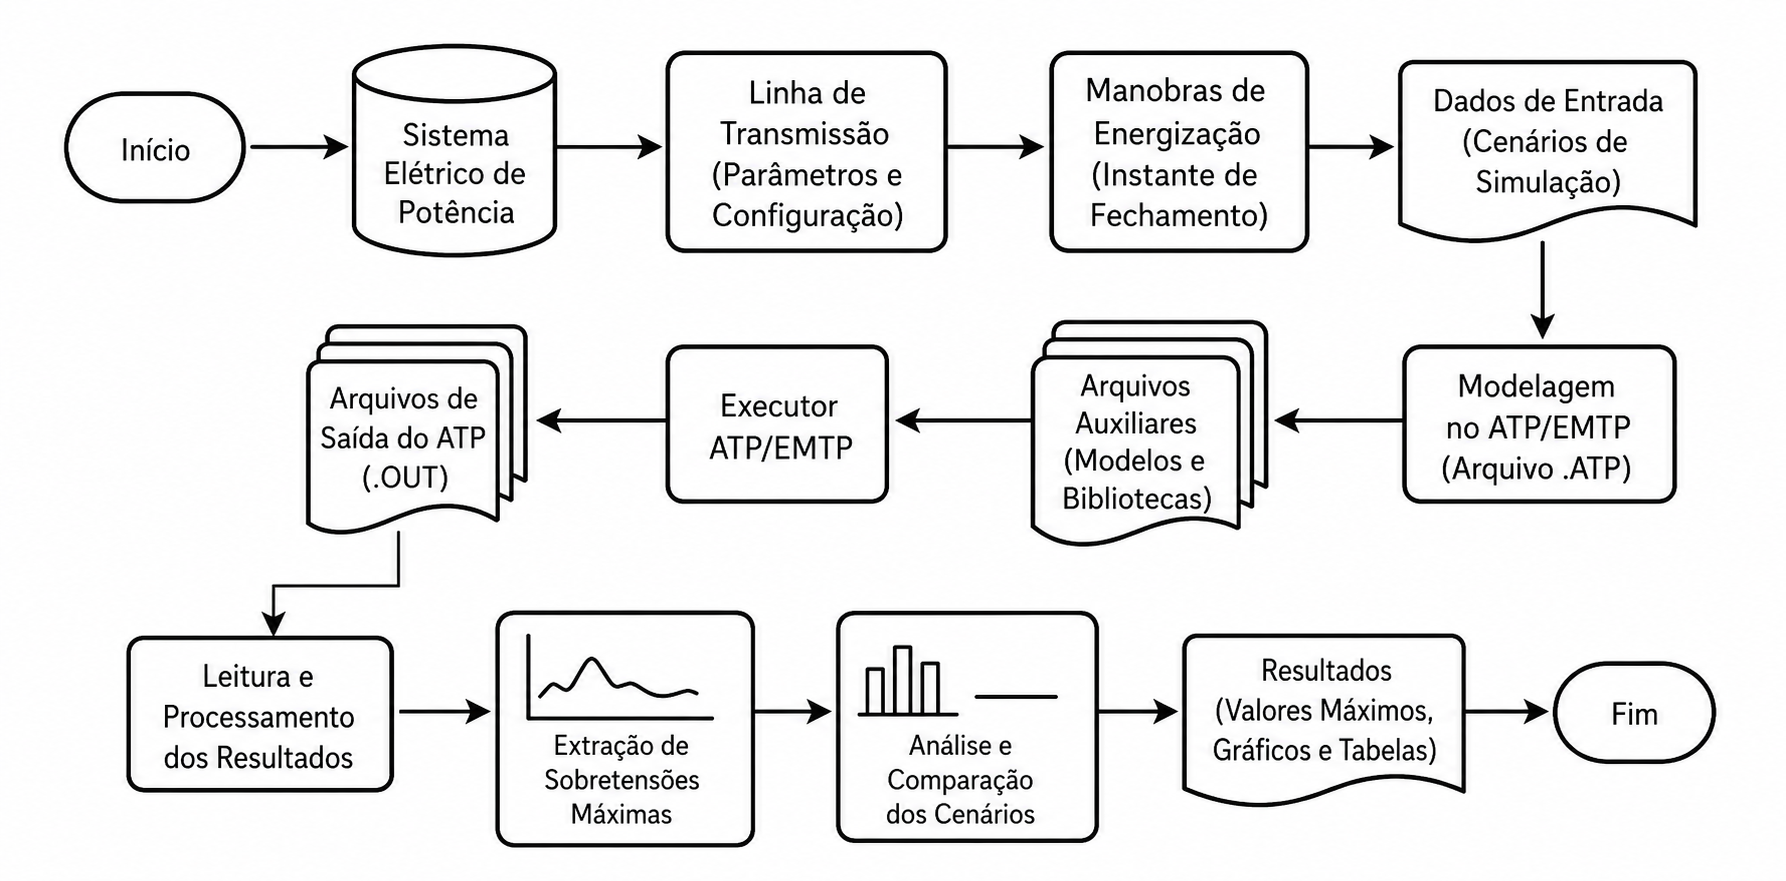
\includegraphics[width=0.75\textwidth]{imagens/fluxo.png}
    \caption{Fluxograma da metodologia de análise de sobretensões transitórias utilizando ATP/EMTP.}
    \label{fig:fluxograma_atp}
\end{figure}

No presente trabalho, esses transitórios são analisados a partir dos valores máximos de sobretensão obtidos em simulações de energização. Esses valores constituem a base de dados utilizada nas etapas posteriores de tratamento estatístico, análise probabilística e detecção de possíveis anomalias.
% \section{Simulação computacional com ATP}
\section{Simulação computacional com ATP e extração dos dados}

O \textit{Alternative Transients Program} (ATP) é uma ferramenta computacional utilizada para a simulação de transitórios eletromagnéticos em sistemas elétricos de potência. Por meio da representação matemática dos componentes do sistema, o programa permite analisar o comportamento de linhas, transformadores, disjuntores, fontes, cargas e demais elementos submetidos a diferentes condições de operação. Em estudos de energização, o ATP possibilita executar múltiplas simulações considerando diferentes instantes de chaveamento e diferentes condições do sistema. A partir dessas simulações, podem ser obtidas as sobretensões máximas em cada fase e em diferentes pontos de monitoramento da linha. De forma complementar, Leão \cite{leao2022} apresenta uma aplicação do ATP na repotencialização de uma linha de transmissão em Manaus-AM, mostrando que o simulador pode ser utilizado para modelar configurações reais de rede e avaliar alternativas técnicas de operação e planejamento. Essa aplicação reforça a importância do ATP como ferramenta de apoio a estudos de linhas de transmissão, especialmente em cenários nos quais a simulação computacional permite avaliar diferentes configurações do sistema e subsidiar decisões técnicas de projeto.

% \section{Extração e organização dos dados do ATP}

Apesar de sua utilidade, a análise dos arquivos gerados pelo ATP pode ser trabalhosa quando há grande volume de simulações, pois os resultados podem estar distribuídos em arquivos extensos, contendo valores numéricos, identificação de fases, pontos de medição e informações de cada execução. Nesse contexto, a automatização da leitura dos arquivos por meio de um \textit{parser} contribui para reduzir o esforço manual, padronizar a extração dos dados e diminuir a possibilidade de erros na organização das informações. Além disso, como as múltiplas simulações produzem um conjunto de valores máximos de tensão, torna-se necessário aplicar procedimentos estatísticos e visuais que permitam compreender a distribuição dos dados, identificar valores extremos e apoiar a interpretação técnica dos resultados.

O código-fonte desenvolvido para o processamento dos dados das linhas de transmissão está disponível em repositório público no GitHub \cite{viana2026repositorio}.

A automatização de estudos envolvendo o ATP também é discutida por Guidi-Venerdini e Pérez-Yauli \cite{guidi2013}, que desenvolveram uma rotina em MATLAB para manipular arquivos-base do ATP e executar simulações sistemáticas em uma linha de transmissão. Embora o foco dos autores esteja na simulação de faltas, o trabalho evidencia a relevância de procedimentos automatizados para a construção de bases de dados, redução do esforço manual e diminuição de erros no tratamento de grandes volumes de resultados.

De forma complementar, Colqui et al. \cite{colqui2022} discutem a implementação de modelos de linhas de transmissão no ATP-EMTP para estudos de transitórios eletromagnéticos, comparando diferentes abordagens de representação, como o modelo JMarti, o \textit{Universal Line Model} e uma implementação modificada do \textit{Folded Line Equivalent}. Os autores avaliam esses modelos em condições de circuito aberto, energização e ocorrência de faltas, evidenciando a importância da escolha adequada da representação da linha para a obtenção de respostas transitórias coerentes. A Figura~\ref{fig:linha_colqui} apresenta um exemplo de sistema de linha de transmissão utilizado nesse tipo de simulação, ilustrando a configuração empregada pelos autores para analisar o comportamento transitório do sistema. Embora o foco do presente trabalho não seja a formulação de novos modelos de linha, a figura reforça a importância da modelagem adequada do sistema elétrico como etapa fundamental para a qualidade dos dados posteriormente analisados.

\begin{figure}[htbp]
    \centering
    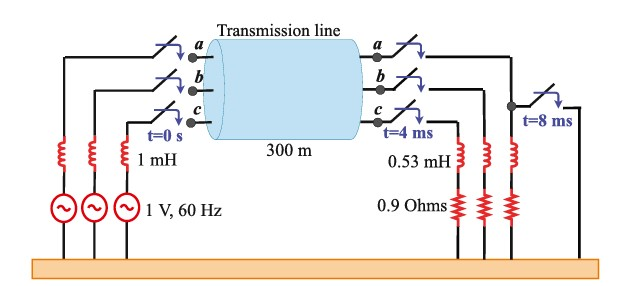
\includegraphics[width=0.75\textwidth]{imagens/linha_transmissao_colqui.jpg}
    \caption{Sistema de linha de transmissão utilizado em simulações de transitórios eletromagnéticos. Fonte: Colqui et al. \cite{colqui2022}.}
    \label{fig:linha_colqui}
\end{figure}

\section{Análise estatística e probabilística dos dados}

A partir dos dados extraídos dos arquivos do ATP, a análise estatística permite descrever e interpretar os valores de sobretensão obtidos nas simulações ou medições, sendo amplamente utilizada em aplicações de engenharia para sintetizar informações, avaliar variabilidade e apoiar decisões técnicas \cite{montgomery2020,devore2016}. Em estudos de sobretensões, ela auxilia na identificação de tendências centrais, dispersão dos valores e ocorrência de eventos extremos. Medidas como média, desvio padrão, mínimo, máximo, quartis e percentis são importantes para compreender o comportamento geral das tensões simuladas. A média fornece uma medida representativa do conjunto analisado, enquanto o desvio padrão expressa o grau de dispersão dos dados em relação a essa média.

Quando os dados apresentam comportamento aproximadamente compatível com uma distribuição normal, a regra empírica de $3\sigma$ pode ser utilizada como critério preliminar para identificação de valores extremos. Por esse critério, valores localizados fora do intervalo

\begin{equation}
[\mu - 3\sigma, \mu + 3\sigma]
\end{equation}
podem ser tratados como candidatos a anomalias ou \textit{outliers}, em que $\mu$ representa a média e $\sigma$ representa o desvio padrão do conjunto de dados. Entretanto, esse critério deve ser aplicado com cautela, pois sua interpretação depende da distribuição dos dados. Em conjuntos assimétricos, multimodais ou com caudas pesadas, a regra de $3\sigma$ pode deixar de representar adequadamente a ocorrência de valores extremos.

Como complemento, podem ser utilizados quartis, percentis e a amplitude interquartil, conhecida como IQR, definida por

\begin{equation}
IQR = Q_3 - Q_1,
\end{equation}
em que $Q_1$ e $Q_3$ representam, respectivamente, o primeiro e o terceiro quartil. Um critério exploratório frequentemente associado ao boxplot considera como candidatos a valores atípicos os pontos situados fora do intervalo

\begin{equation}
[Q_1 - 1{,}5IQR, Q_3 + 1{,}5IQR].
\end{equation}
Esse procedimento não substitui a interpretação física do fenômeno, mas oferece uma referência adicional para identificar observações que se afastam da região central dos dados.

A análise probabilística complementa a descrição estatística ao permitir estimar a frequência de ocorrência de eventos críticos. Considerando $N$ simulações e um limiar de sobretensão $v$, a probabilidade empírica de excedência pode ser estimada por

\begin{equation}
\hat{P}(V > v)=\frac{n_v}{N},
\end{equation}
em que $n_v$ representa o número de observações cujo valor de sobretensão $V$ excede o limiar estabelecido. Essa estimativa permite avaliar, por exemplo, a proporção de simulações que ultrapassa determinado nível de tensão. Quando necessário, níveis de confiança podem ser associados a estimativas proporcionais por meio de aproximações estatísticas, como

\begin{equation}
IC_{\hat{p}} = \hat{p} \pm z_{\alpha/2}\sqrt{\frac{\hat{p}(1-\hat{p})}{N}},
\end{equation}
em que $\hat{p}$ representa a proporção estimada, $z_{\alpha/2}$ é o valor crítico da distribuição normal padrão e $N$ é o número total de observações. A identificação de \textit{outliers}, entretanto, deve ser conduzida com cautela, pois valores discrepantes podem ter diferentes origens e interpretações, não sendo necessariamente erros ou observações inválidas \cite{barnett1994}. Em aplicações de sistemas elétricos, um valor extremo pode representar um evento fisicamente relevante, uma condição operacional rara, um comportamento transitório específico ou, ainda, um desvio associado ao processo numérico da simulação. Portanto, a análise estatística e probabilística deve ser combinada com visualização de dados, interpretação física e métodos computacionais de identificação de padrões.

\section{Visualização de dados e análise exploratória}

A visualização de dados constitui uma etapa importante da análise exploratória, pois permite observar padrões, agrupamentos, dispersões e valores discrepantes que nem sempre são identificados apenas por medidas numéricas. Tukey \cite{tukey1977} destaca a análise exploratória como parte essencial da compreensão dos dados. Cleveland \cite{cleveland1993} ressalta que a visualização permite investigar a estrutura dos dados e revelar comportamentos relevantes para a análise. De forma complementar, Tufte \cite{tufte2001} enfatiza que bons gráficos devem comunicar informações quantitativas com clareza, precisão e eficiência. Entre as formas mais utilizadas de visualização está a nuvem de pontos, ou \textit{scatter plot}. Nesse tipo de gráfico, cada ponto representa uma observação posicionada de acordo com duas variáveis de interesse. No contexto deste trabalho, cada ponto pode representar uma simulação, uma fase monitorada, um ponto de medição ou uma combinação de atributos extraídos dos arquivos do ATP. Essa representação permite observar concentrações de valores, regiões de dispersão, possíveis agrupamentos e pontos isolados.

A Figura~\ref{fig:nuvem-clusters-anomalias} apresenta uma representação esquemática de uma nuvem de pontos com agrupamentos e possíveis observações anômalas. Os centróides representam os centros dos grupos, conceito associado a métodos particionais como o K-Means, enquanto os pontos afastados das regiões de maior concentração podem ser analisados como candidatos a valores atípicos. No presente trabalho, a visualização por nuvem de pontos será utilizada como ferramenta de apoio à análise das sobretensões máximas obtidas nas simulações. Antes da aplicação dos algoritmos, ela permite observar a distribuição geral dos dados e identificar visualmente concentrações ou valores extremos. Após a aplicação dos métodos estatísticos e de aprendizagem de máquina, contribui para interpretar os agrupamentos formados e a posição dos pontos classificados como possíveis anomalias.

\begin{figure}[htbp]
\centering
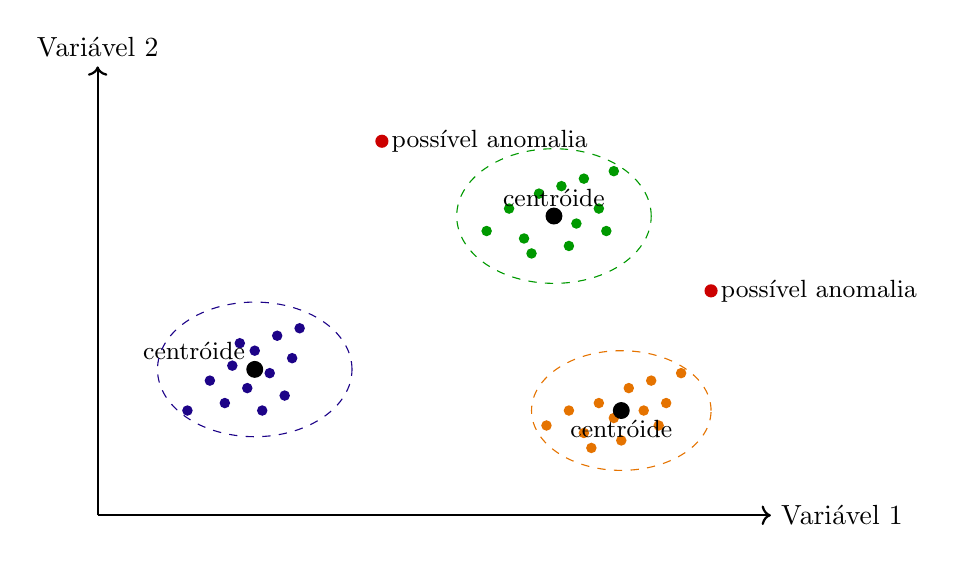
\begin{tikzpicture}[scale=0.95]

% Eixos
\draw[->, thick] (0,0) -- (9,0) node[right] {Variável 1};
\draw[->, thick] (0,0) -- (0,6) node[above] {Variável 2};

% Cluster 1
\foreach \x/\y in {
1.2/1.4,1.5/1.8,1.7/1.5,1.8/2.0,2.0/1.7,
2.1/2.2,2.3/1.9,2.4/2.4,2.6/2.1,2.7/2.5,
2.2/1.4,1.9/2.3,2.5/1.6}
\fill[blue!70!black] (\x,\y) circle (2pt);

% Cluster 2
\foreach \x/\y in {
5.2/3.8,5.5/4.1,5.7/3.7,5.9/4.3,6.1/4.0,
6.2/4.4,6.4/3.9,6.5/4.5,6.7/4.1,6.9/4.6,
5.8/3.5,6.3/3.6,6.8/3.8}
\fill[green!60!black] (\x,\y) circle (2pt);

% Cluster 3
\foreach \x/\y in {
6.0/1.2,6.3/1.4,6.5/1.1,6.7/1.5,6.9/1.3,
7.1/1.7,7.3/1.4,7.4/1.8,7.6/1.5,7.8/1.9,
6.6/0.9,7.0/1.0,7.5/1.2}
\fill[orange!90!black] (\x,\y) circle (2pt);

% Centroides
\filldraw[black] (2.1,1.95) circle (3pt);
\filldraw[black] (6.1,4.0) circle (3pt);
\filldraw[black] (7.0,1.4) circle (3pt);

\node[above left] at (2.1,1.95) {\small centróide};
\node[above] at (6.1,4.0) {\small centróide};
\node[below] at (7.0,1.4) {\small centróide};

% Possíveis anomalias
\fill[red!80!black] (3.8,5.0) circle (2.5pt);
\fill[red!80!black] (8.2,3.0) circle (2.5pt);
\node[right] at (3.8,5.0) {\small possível anomalia};
\node[right] at (8.2,3.0) {\small possível anomalia};

% Contornos dos grupos
\draw[dashed, blue!70!black] (2.1,1.95) ellipse (1.3 and 0.9);
\draw[dashed, green!60!black] (6.1,4.0) ellipse (1.3 and 0.9);
\draw[dashed, orange!90!black] (7.0,1.4) ellipse (1.2 and 0.8);

\end{tikzpicture}
\caption{Representação esquemática de uma nuvem de pontos com agrupamentos identificados e possíveis observações anômalas. Fonte: elaboração própria.}
\label{fig:nuvem-clusters-anomalias}
\end{figure}


\section{Detecção de anomalias e aprendizagem de máquina em sistemas elétricos}

A detecção de anomalias consiste na identificação de observações que se diferenciam significativamente do comportamento predominante de um conjunto de dados. Essas observações também podem ser chamadas de \textit{outliers}, valores atípicos ou pontos discrepantes. Em bases numéricas, anomalias podem surgir por erros de medição, falhas de processamento, ruídos, eventos raros ou comportamentos reais de interesse para o estudo. No contexto deste trabalho, a detecção de anomalias está relacionada à identificação de sobretensões máximas que se afastam do padrão observado nas simulações de energização de linhas de transmissão. Esses valores exigem atenção, pois podem influenciar a interpretação dos resultados estatísticos e afetar a estimativa dos níveis de isolamento. Um único valor extremo, quando tratado sem análise adequada, pode conduzir a conclusões excessivamente conservadoras ou tecnicamente inconsistentes. Assim, a classificação de uma sobretensão como anômala não significa, necessariamente, que ela deva ser descartada. O processo de análise deve considerar se o valor possui coerência com o comportamento físico esperado, se ocorre de forma repetida em condições semelhantes e se está associado a uma configuração plausível do sistema simulado.

A aprendizagem de máquina, ou \textit{Machine Learning}, é uma área da Inteligência Artificial dedicada ao desenvolvimento de métodos capazes de reconhecer padrões e extrair informações a partir de dados. Segundo Mitchell \cite{mitchell1997}, um programa computacional aprende a partir da experiência quando seu desempenho em determinada tarefa melhora em função dessa experiência. De modo geral, os métodos de aprendizagem de máquina podem ser classificados em aprendizagem supervisionada, aprendizagem não supervisionada e aprendizagem por reforço. Na aprendizagem supervisionada, os dados possuem rótulos previamente conhecidos. Na aprendizagem não supervisionada, os dados não possuem classificação prévia, e o objetivo é identificar estruturas internas, padrões de similaridade, agrupamentos ou observações discrepantes. Já a aprendizagem por reforço envolve a tomada de decisões sequenciais por um agente que aprende a partir de recompensas ou penalizações recebidas em sua interação com o ambiente. No contexto deste trabalho, destaca-se a aprendizagem não supervisionada, pois os dados provenientes das simulações realizadas no ATP não apresentam, inicialmente, uma classificação prévia que indique quais sobretensões devem ser consideradas normais, críticas ou anômalas. Assim, técnicas não supervisionadas tornam-se adequadas para apoiar a análise exploratória da base de dados, permitindo reconhecer padrões predominantes e sinalizar observações que se afastam do comportamento global do conjunto analisado.

A aplicação de técnicas de aprendizagem de máquina em sistemas elétricos tem crescido em diferentes frentes, incluindo previsão de carga, identificação de falhas, análise de estabilidade, monitoramento de redes inteligentes, detecção de ataques cibernéticos e reconhecimento de padrões anômalos em dados operacionais. Guato Burgos, Morato e Vizcaino Imacaña \cite{guato2024} apresentam uma revisão sobre abordagens de detecção de anomalias em redes elétricas inteligentes baseadas em técnicas de Inteligência Artificial, destacando aplicações relacionadas a falhas, irregularidades em medições, ataques cibernéticos e padrões operacionais incomuns. Aghazadeh Ardebili et al. \cite{ardebili2024} realizam uma revisão sistemática sobre detecção de anomalias em tempo real em sistemas energéticos complexos, destacando sua importância para a resiliência operacional dessas infraestruturas. Khaledian et al. \cite{khaledian2021} aplicam métodos como Isolation Forest, K-Means e LoOP à detecção e classificação de anomalias em dados sincrofasoriais em tempo real, enquanto Ren, Hou e Etingov \cite{ren2018} investigam a detecção de anomalias no contexto da estimação de estado em sistemas de potência. Gillioz et al. \cite{gillioz2026}, por sua vez, aplicam algoritmos de aprendizagem de máquina à detecção de anomalias em dados operacionais de redes elétricas de grande porte e alta tensão, evidenciando que métodos baseados em dados podem apoiar a identificação de comportamentos incomuns em sistemas de transmissão. Embora esses estudos não estejam diretamente voltados à análise de sobretensões transitórias geradas por simulações no ATP, eles fornecem suporte conceitual e metodológico para a proposta deste trabalho, pois a identificação de anomalias em sobretensões simuladas compartilha desafios semelhantes, como tratamento de grandes volumes de dados, reconhecimento de padrões predominantes e distinção entre valores extremos relevantes e observações discrepantes.

\section{Aprendizagem de máquina não supervisionada e clusterização}

Entre os métodos de aprendizagem não supervisionada, os algoritmos de clusterização ocupam posição de destaque. A clusterização tem como objetivo organizar observações em grupos, de modo que elementos pertencentes ao mesmo grupo apresentem maior similaridade entre si do que em relação a elementos de outros grupos \cite{bishop2006}. No caso das sobretensões obtidas em manobras de energização de linhas de transmissão, os algoritmos de clusterização podem auxiliar na identificação de faixas de comportamento recorrentes e na separação de valores discrepantes. Cada observação pode representar uma simulação, uma fase monitorada, um ponto de medição ou um valor máximo de tensão. A partir desses atributos, torna-se possível analisar se as sobretensões se organizam em grupos coerentes ou se existem valores isolados que devem ser investigados como possíveis anomalias.

\subsection{K-Means}

O K-Means é um algoritmo clássico de clusterização não supervisionada. O método foi introduzido por MacQueen \cite{macqueen1967}, no contexto da classificação e análise de observações multivariadas, com o objetivo de particionar uma população ou amostra em $k$ conjuntos com baixa variabilidade interna. Posteriormente, o procedimento iterativo de atribuição de pontos aos representantes mais próximos e atualização desses representantes foi associado ao algoritmo de Lloyd, originalmente formulado no contexto de quantização por mínimos quadrados \cite{lloyd1982}. O K-Means divide um conjunto de dados em $k$ agrupamentos, sendo $k$ definido previamente pelo usuário. Cada agrupamento é representado por um centróide, calculado como a média das observações pertencentes ao grupo. O algoritmo alterna duas etapas principais: atribuição de cada ponto ao centróide mais próximo e atualização dos centróides com base na média dos pontos atribuídos a cada grupo. Esse processo se repete até a estabilização dos agrupamentos. Matematicamente, o K-Means procura minimizar a soma das distâncias quadráticas entre cada observação e o centróide do grupo ao qual ela pertence:

\begin{equation}
J = \sum_{j=1}^{k} \sum_{x_i \in C_j} |x_i - \mu_j|^2,
\end{equation}
em que $C_j$ representa o $j$-ésimo agrupamento, $\mu_j$ é o centróide desse agrupamento e $x_i$ representa uma observação da base de dados \cite{bishop2006}. Mahon e Lapata \cite{mahon2025} destacam que, apesar de sua simplicidade, o K-Means permanece como um dos algoritmos de clusterização mais utilizados, devido à sua rapidez, à garantia de convergência, à existência de um parâmetro de fácil interpretação e ao desempenho competitivo em relação a métodos mais complexos. Entretanto, os autores também ressaltam como limitação a necessidade de definir previamente o número de clusters $k$. Essa limitação é relevante para este trabalho, pois, em bases de dados provenientes de simulações de transitórios eletromagnéticos, nem sempre se conhece previamente a quantidade ideal de padrões ou grupos de comportamento existentes.

Mahon e Lapata \cite{mahon2025} apresentam uma aplicação baseada em métodos de clusterização associados ao K-Means, observada na Figura~\ref{fig:kmeans-mahon}. A figura apresenta dados sintéticos com 20 agrupamentos em diferentes níveis de separação entre os centróides. À esquerda, os grupos estão mais sobrepostos; ao centro, apresentam separação intermediária; à direita, encontram-se mais bem definidos. Essa representação evidencia que o desempenho de métodos baseados em centróides depende da distribuição dos dados no espaço de atributos. Quando os grupos são compactos e bem separados, a identificação dos agrupamentos tende a ser mais clara. Entretanto, quando há sobreposição, dispersão elevada ou proximidade entre centróides, a clusterização torna-se mais sensível à escolha de $k$, à inicialização dos centróides e ao pré-processamento dos dados. No presente trabalho, o K-Means será utilizado como ferramenta exploratória para verificar se as sobretensões máximas obtidas nas simulações se organizam em grupos de comportamento semelhante. Pontos muito distantes dos centróides ou pertencentes a grupos pouco representativos podem ser analisados como possíveis candidatos a anomalias.

\begin{figure}[htbp]
\centering
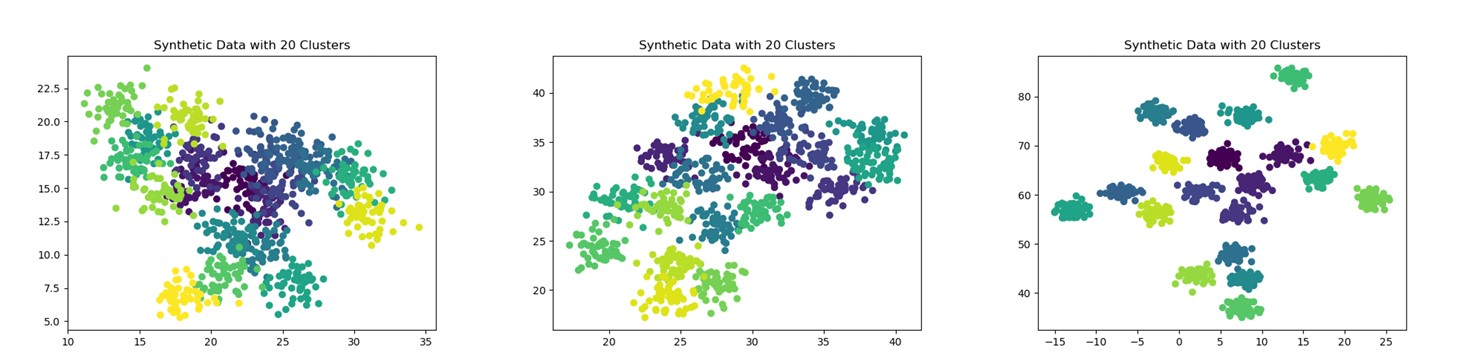
\includegraphics[width=\textwidth]{kmeans.jpg}
\caption{Aplicação de clusterização baseada em K-Means em dados sintéticos com 20 agrupamentos e diferentes níveis de separação entre centróides. Fonte: Mahon e Lapata \cite{mahon2025}.}
\label{fig:kmeans-mahon}
\end{figure}

\subsection{DBSCAN}

O DBSCAN, sigla para \textit{Density-Based Spatial Clustering of Applications with Noise}, foi proposto por Ester et al. \cite{ester1996} para identificar agrupamentos em grandes bases de dados espaciais com presença de ruído. Diferentemente do K-Means, o DBSCAN não exige a definição prévia do número de grupos. O método baseia-se na densidade local dos pontos, permitindo identificar clusters com formatos arbitrários e classificar como ruído os pontos localizados em regiões pouco densas. O algoritmo utiliza dois parâmetros principais: $\varepsilon$, que define o raio de vizinhança ao redor de um ponto, e \textit{MinPts}, que indica o número mínimo de pontos necessário para que uma região seja considerada densa. A vizinhança de raio $\varepsilon$ de um ponto $p$ é definida por

\begin{equation}
N_{\varepsilon}(p)={q \in D \mid dist(p,q)\leq \varepsilon},
\end{equation}
em que $D$ representa a base de dados e $dist(p,q)$ corresponde à função de distância entre os pontos $p$ e $q$. Com base nessa vizinhança, os pontos são classificados como centrais, de borda ou ruído. Um ponto central possui pelo menos \textit{MinPts} observações em sua vizinhança. Um ponto de borda não possui vizinhos suficientes para ser central, mas está localizado na vizinhança de um ponto central. Um ponto de ruído não é central e não pertence à vizinhança de nenhum ponto central. O funcionamento do DBSCAN ocorre pela expansão de agrupamentos: inicialmente, o algoritmo seleciona um ponto ainda não visitado e verifica sua vizinhança; se o ponto satisfaz a condição de ponto central, inicia-se um novo cluster, incorporando todos os pontos direta ou indiretamente alcançáveis por densidade; caso contrário, o ponto pode ser classificado como ruído. O processo é repetido até que todos os pontos da base tenham sido avaliados.

Mumtaz e Duraiswamy \cite{mumtaz2010} comparam o desempenho do DBSCAN, do K-Means e dos Mapas Auto-Organizáveis de Kohonen, conhecidos como SOM, em bases sintéticas espaciais. A comparação evidencia que o DBSCAN apresenta melhor desempenho em conjuntos de dados com formatos arbitrários, não convexos e estruturas espiraladas. Enquanto o K-Means tende a separar os dados em grupos influenciados pela proximidade aos centróides, o DBSCAN preserva melhor a forma natural dos agrupamentos, pois sua definição de cluster depende da densidade local dos pontos. A Figura~\ref{fig:dbscan-comparacao} apresenta uma comparação entre os resultados de clusterização obtidos por SOM, K-Means e DBSCAN em bases sintéticas bidimensionais. Essa característica é importante para a detecção de anomalias, pois o DBSCAN não força todos os pontos a pertencerem a algum grupo. Pontos situados em regiões de baixa densidade podem ser classificados como ruído, tornando o método adequado para identificar observações que não seguem o comportamento predominante da base de dados. No contexto deste trabalho, o DBSCAN será utilizado para auxiliar na identificação de sobretensões máximas isoladas em relação ao conjunto analisado. Entretanto, uma observação classificada como ruído não deve ser descartada automaticamente. Sua interpretação deve considerar a análise estatística, os parâmetros da simulação e a coerência física do fenômeno transitório.

\begin{figure}[htbp]
\centering
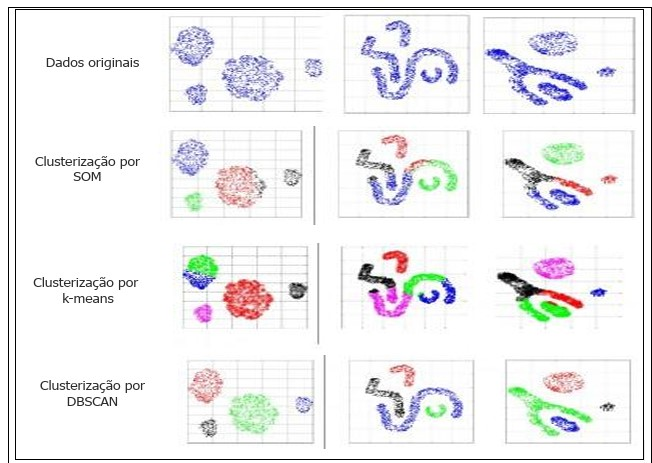
\includegraphics[width=\textwidth]{dbscan.jpg}
\caption{Comparação entre os resultados de clusterização obtidos por SOM, K-Means e DBSCAN em dados espaciais sintéticos. Fonte: adaptado de Mumtaz e Duraiswamy \cite{mumtaz2010}, reproduzido em documento da Biblioteca Digital Maxwell/PUC-Rio \cite{maxwell2014}.}
\label{fig:dbscan-comparacao}
\end{figure}

Apesar de suas vantagens, o DBSCAN apresenta limitações. A escolha inadequada de $\varepsilon$ ou de \textit{MinPts} pode levar à fragmentação excessiva dos agrupamentos ou à classificação indevida de muitos pontos como ruído. Além disso, quando os dados apresentam regiões com densidades muito diferentes, o uso de parâmetros globais pode dificultar a identificação correta dos clusters. Por isso, sua aplicação deve ser acompanhada de análise exploratória, visualização gráfica e validação técnica.

Com base nos conceitos apresentados, observa-se que a análise de sobretensões transitórias em manobras de energização exige a integração entre conhecimento físico do sistema elétrico, simulação computacional, tratamento estatístico, análise probabilística e técnicas de reconhecimento de padrões. O ATP fornece os dados necessários para representar diferentes condições de operação, enquanto a estatística e a visualização auxiliam na compreensão da distribuição dos valores máximos obtidos. Os algoritmos de clusterização, por sua vez, podem apoiar a identificação de comportamentos predominantes e de observações discrepantes. Essa fundamentação sustenta a etapa metodológica do trabalho, na qual serão definidos os procedimentos de extração, organização, análise probabilística e classificação das sobretensões simuladas.

\chapter{Modelagem do sistema elétrico}

Este capítulo descreve o sistema elétrico utilizado para gerar os dados
sintéticos analisados neste trabalho. Seu objetivo não é desenvolver um novo
modelo de rede nem realizar um estudo completo de planejamento elétrico, mas
registrar a origem dos dados, as simplificações adotadas e as variáveis que
podem influenciar as sobretensões obtidas. Essa descrição estabelece a
rastreabilidade entre o cenário elétrico, os arquivos produzidos pelo ATP e a
base posteriormente processada pela aplicação em Python.

O nível de detalhamento foi limitado às decisões necessárias para compreender
e reproduzir o processo de geração dos dados. Assim, são apresentados o caso
de referência, a redução da rede, a representação dos componentes no ATPDraw,
o modelo da linha de transmissão e os pontos de observação, sem aprofundar as
formulações matemáticas próprias dos programas elétricos empregados.

\section{Dados de entrada e cenário de referência}

O ponto de partida foi um caso do Sistema Interligado Nacional disponibilizado
pelo Operador Nacional do Sistema Elétrico (ONS) para o ciclo PAR/PEL
2027--2031. Foi selecionado o cenário de inverno de 2031, no patamar de carga
máxima noturna. A base de fluxo de potência foi fornecida no formato do
ANAREDE, enquanto o caso de curto-circuito utilizado corresponde ao arquivo
\texttt{BR2612PJ.ANA}, configuração de dezembro de 2026 e versão de 31 de
março de 2026.

As duas bases desempenham funções distintas e complementares. O ANAREDE é
utilizado para estudos de regime permanente e fornece o ponto de operação do
sistema, incluindo níveis de tensão, carregamentos e condições de geração. O
ANAFAS é destinado a estudos de curto-circuito e fornece os parâmetros
necessários à representação da resposta da rede diante de perturbações
\cite{cepelAnarede2026,cepelAnafas2026}. O uso conjunto dessas informações é
compatível com a prática adotada nos estudos do PAR/PEL, que disponibilizam
casos de fluxo de potência e de curto-circuito para os programas da plataforma
CEPEL \cite{ons2026pnast}.

Essa identificação do cenário é relevante para a análise computacional porque
os valores produzidos pelo ATP não constituem medições de campo. Eles são
dados sintéticos condicionados pelo estado inicial e pelos parâmetros do caso
selecionado. Consequentemente, qualquer comparação entre simulações deve manter
o cenário de referência ou registrar explicitamente suas alterações.

\section{Redução da rede}

A representação integral do Sistema Interligado Nacional introduziria grande
quantidade de elementos sem relação direta com a manobra investigada. Para
delimitar uma região de estudo controlada, foi empregada a função de cálculo de
equivalentes do ANAFAS. O programa permite substituir a parcela externa da rede
por ligações equivalentes, com erro máximo definido durante o procedimento de
redução \cite{cepelAnafas2026}.

No modelo resultante, foram preservadas as barras e os equipamentos da região
de interesse, enquanto a influência do restante do sistema foi representada
por equivalentes série e em derivação conectados às barras de fronteira. As
três conexões equivalentes visíveis no diagrama representam a interação com a
rede externa; elas não devem ser confundidas com a quantidade total de
barramentos do modelo. A rede reduzida ainda contém barras nos níveis de
500~kV, 345~kV, 138~kV e 13,8~kV, além dos nós auxiliares necessários à
representação dos transformadores.

Essa redução procura conservar, nas fronteiras escolhidas, o comportamento de
curto-circuito considerado pelo ANAFAS. Ela não implica que todas as
características transitórias da rede completa sejam preservadas. Essa
limitação é importante para a interpretação dos dados: uma observação atípica
deve ser investigada em relação ao modelo reduzido e às suas condições de
simulação antes de ser associada a um fenômeno da rede real.

\section{Componentes da rede reduzida}

A Figura~\ref{fig:equivalente_anafas} apresenta o diagrama unifilar da região
equivalentada. Entre os elementos mantidos encontram-se quatro
transformadores, a interligação existente entre as barras de 138~kV e os
equipamentos associados às subestações representadas. Três fontes equivalentes
conectam a área preservada ao restante do sistema. Os rótulos das barras foram
mantidos durante a conversão para permitir a conferência entre os arquivos do
ONS, o diagrama do ANAFAS e o modelo do ATPDraw.

\begin{figure}[htbp]
    \centering
    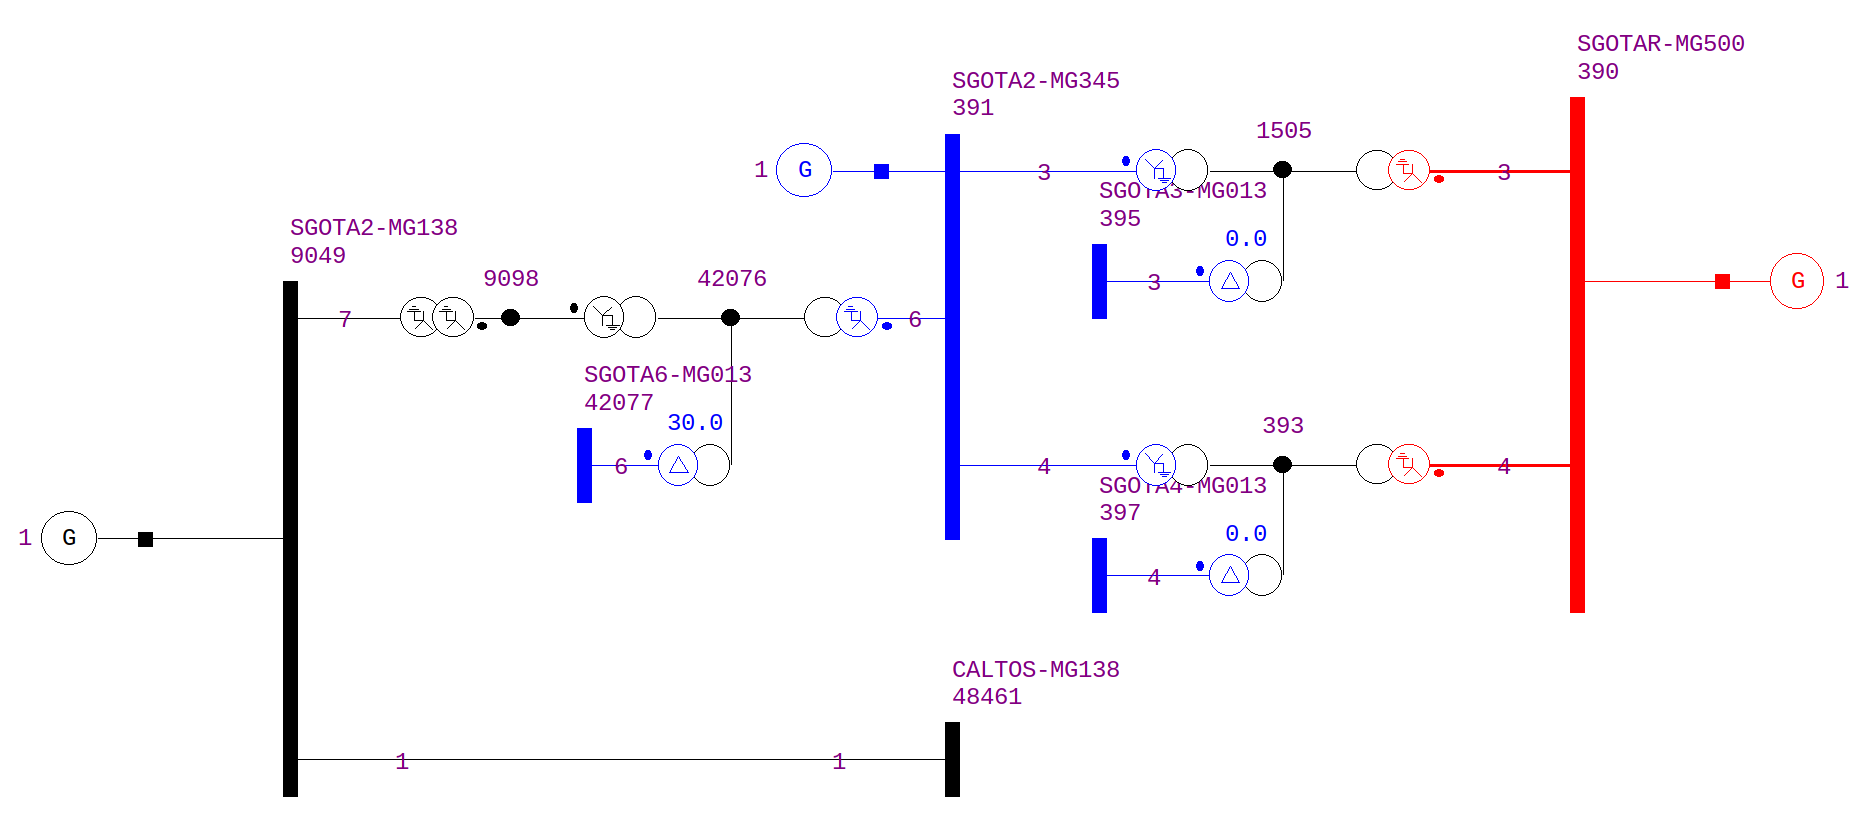
\includegraphics[width=0.95\textwidth]{imagens/rede_equivalente_anafas.png}
    \caption{Rede elétrica equivalente representada no ANAFAS. Fonte:
    elaboração própria a partir da base do ONS.}
    \label{fig:equivalente_anafas}
\end{figure}

\section{Rede modelada no ATPDraw}

Após a redução, os componentes foram representados no ATPDraw para a execução
das simulações de transitórios eletromagnéticos. A conversão exigiu associar
cada elemento da rede de origem a um componente compatível do ATP. A
Tabela~\ref{tab:mapeamento-atpdraw} resume esse mapeamento e sua relação com os
dados gerados.

\begin{table}[htbp]
\centering
\caption{Mapeamento dos principais elementos para o ATPDraw.}
\label{tab:mapeamento-atpdraw}
\begin{tabularx}{\textwidth}{L L L}
\hline
\textbf{Informação de origem} &
\textbf{Representação no ATPDraw} &
\textbf{Relação com os dados} \\
\hline
Ponto de operação do ANAREDE &
Fontes e condições iniciais &
Define as tensões anteriores à manobra \\

Rede externa equivalente &
Fontes e impedâncias equivalentes &
Representa a influência do sistema externo \\

Transformadores &
Transformadores trifásicos e suas ligações &
Conecta os diferentes níveis de tensão \\

Linha sob estudo &
Modelo de parâmetros distribuídos &
Determina a propagação das ondas de tensão \\

Disjuntor de manobra &
Chaves estatísticas por fase &
Varia os instantes de energização \\

Pontos de medição &
Sondas de tensão &
Produz os valores processados pela aplicação \\
\hline
\end{tabularx}
\end{table}

A Figura~\ref{fig:equivalente_atp_draw} mostra a implementação da rede
equivalente. As identificações das barras foram preservadas para facilitar a
verificação do modelo e a associação dos resultados a cada configuração. A
linha submetida à energização foi conectada entre as proximidades das barras
9049 e 48461, pertencentes ao nível de 138~kV. Os terminais e os pontos
intermediários receberam nomes próprios, empregados posteriormente pelo
\textit{parser} para reconhecer as variáveis nos arquivos de saída.

\begin{figure}[htbp]
    \centering
    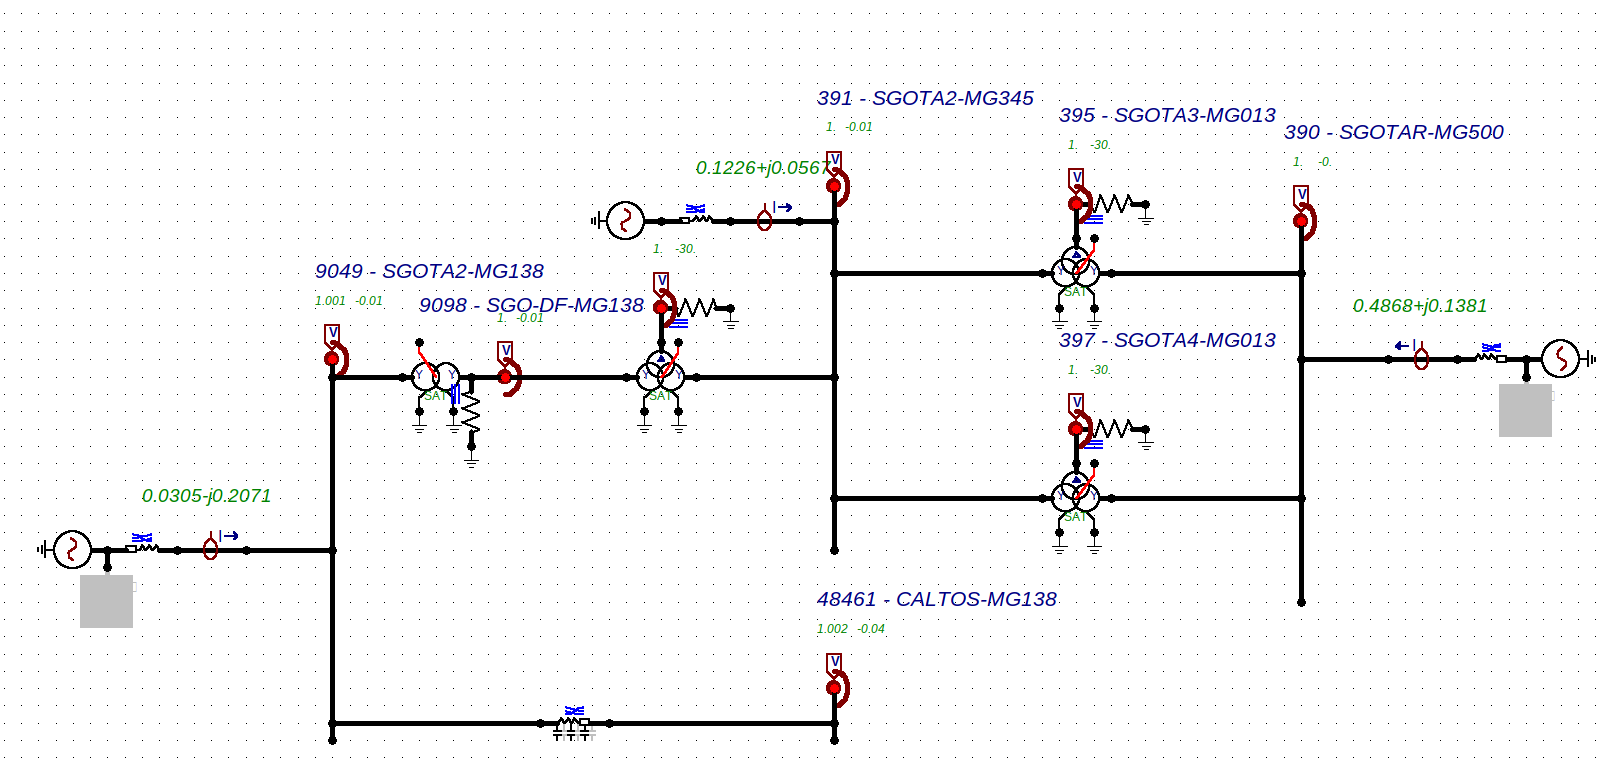
\includegraphics[width=0.95\textwidth]{imagens/rede_equivalente_atp_draw.png}
    \caption{Rede elétrica equivalente implementada no ATPDraw. Fonte:
    elaboração própria.}
    \label{fig:equivalente_atp_draw}
\end{figure}

\section{Modelo da linha de transmissão}

A linha de transmissão analisada possui tensão nominal de 138~kV e extensão
total de 80~km. No ATPDraw, ela foi representada pelo modelo K.C. Lee não
transposto, cujos parâmetros foram calculados a 60~Hz. A representação também
considera a disposição geométrica dos condutores e a resistividade do solo de
$1000~\Omega\cdot\text{m}$. Esses dados afetam a propagação e a reflexão das
ondas eletromagnéticas e, portanto, influenciam diretamente os valores máximos
registrados durante a energização.

Para permitir a observação espacial das sobretensões, a linha foi dividida em
quatro trechos: dois trechos externos de 13,3~km e dois trechos internos de
26,7~km. A soma das extensões resulta nos 80~km do circuito. Essa divisão
introduz um ponto de medição no centro da linha sem alterar sua continuidade
elétrica. A Figura~\ref{fig:modelo_linha} apresenta essa organização.

\begin{figure}[htbp]
    \centering
    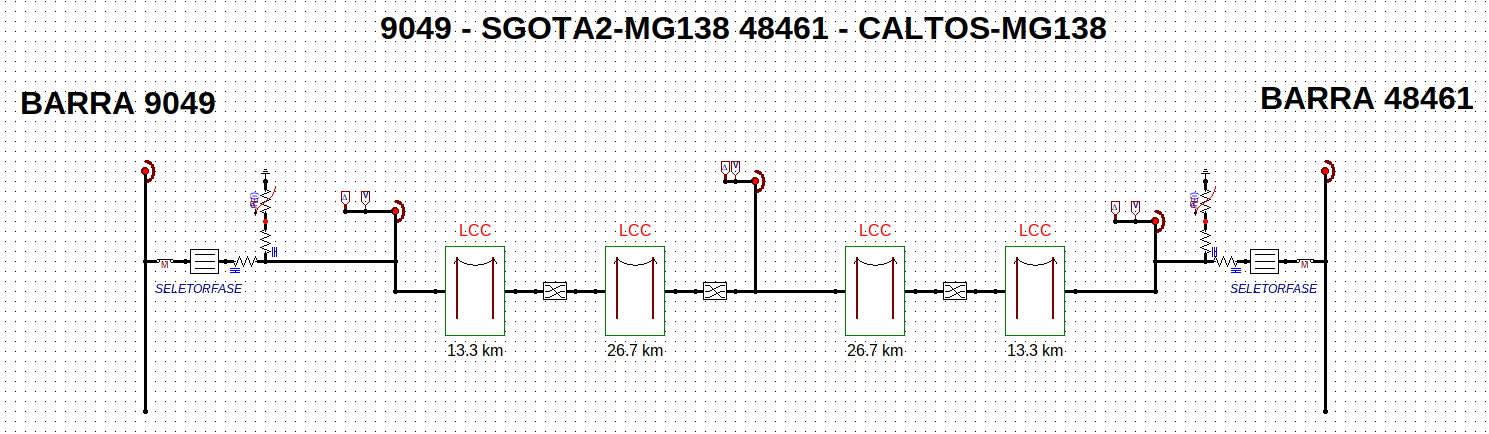
\includegraphics[width=\textwidth]
        {imagens/modelo_linha_transmissão.png}
    \caption{Linha de transmissão modelada no ATPDraw, com quatro trechos e
    pontos de observação ao longo do circuito. Fonte: elaboração própria.}
    \label{fig:modelo_linha}
\end{figure}

As tensões fase-terra são registradas nas três fases nos pontos
$T_{MAN}$, $1/2\,LT$ e $T_{OPO}$. O primeiro corresponde ao terminal onde é
realizada a manobra, o segundo representa o centro elétrico da linha e o
terceiro corresponde ao terminal oposto. Essa nomenclatura também aparece nos
arquivos do ATP como \texttt{T\_MAN}, \texttt{1\_2LT} e \texttt{T\_OPO},
estabelecendo uma correspondência direta entre o modelo e as colunas da base
processada.

\section{Manobra e geração dos dados}

A energização é executada por chaves estatísticas independentes para as fases
A, B e C. Em vez de utilizar um único instante determinístico, o ATP produz
múltiplas execuções com pequenas variações nos tempos de fechamento. Dessa
forma, cada execução representa uma possível condição de manobra e gera um
conjunto de valores máximos de tensão. O modelo também permite comparar
configurações com e sem resistor de pré-inserção, além de diferentes
representações da rede equivalente.

Nos casos examinados, o passo de integração é de $10~\mu\text{s}$ e a janela
simulada é de 0,3~s. Ao final de cada execução, o ATP registra no arquivo de
saída a identificação da simulação, o ponto monitorado, a fase, o valor máximo
e o instante em que esse máximo ocorreu. A quantidade de execuções é um
parâmetro do experimento; por isso, foram preparados conjuntos com 50, 100,
200, 1.000 e 10.000 simulações estatísticas para avaliar também o efeito do
tamanho da amostra.

Esses arquivos constituem a entrada da etapa computacional deste trabalho. O
\textit{parser} associa os nomes dos terminais e das fases aos valores extraídos
e transforma cada máximo observado em um registro estruturado. Assim, o fluxo
de dados pode ser resumido como: caso do ONS, rede equivalente, modelo no ATP,
simulações estatísticas, arquivos de saída e base tabular analisada em Python.

\subsection{Escopo e validação do parser}

O reconhecimento do arquivo estatístico utiliza os marcadores textuais
\texttt{NENERG}, \texttt{otherwise blank space}, a identificação numerada de
cada simulação e a tabela \texttt{Times of maxima}. Para cada execução, são
preservados o identificador, os tempos de chaveamento, o sinal do máximo, o
instante de ocorrência e a associação com o cabeçalho da variável. Arquivos
estatísticos com cabeçalho ausente, numeração descontínua, quantidade de
execuções divergente de \texttt{NENERG} ou comprimentos incompatíveis entre
máximos e tempos são rejeitados. Arquivos \texttt{.lis} sem \texttt{NENERG}
são tratados como saídas não estatísticas e não geram observações.

Uma auditoria de fidelidade às fontes foi ampliada em 10 de setembro de 2026,
após a identificação de um defeito de alinhamento do cabeçalho do CRPI. A
separação dos nomes dos nós por espaços em branco removia células vazias e
associava nós de ramificação às variáveis incorretas. O parser corrigido utiliza
as posições impressas das colunas de variáveis para preservar células vazias no
início, no interior e no final dos nós. Um caso de regressão sintético
reproduz a falha original e verifica o mapeamento corrigido.

O escopo avaliado dos pontos de verificação das fontes compreende
\texttt{T\_MAN/\{SRPI,CRPI\}/CASO-COMPLETO/SDEF}, com 50, 100, 200,
1.000 e 10.000 simulações por cenário. A referência do CRPI registra todos os
48 pares ordenados de variável/nó, transcritos das linhas 1.784--1.797 da
e compara esses pares nos cinco arquivos. As primeiras e últimas execuções
fornecem os máximos com sinal e os instantes de ocorrência da fase A em
$T_{MAN}$, $1/2\,LT$ e $T_{OPO}$, juntamente com os instantes da chave 10. As
referências são lidas diretamente do texto do ATP, de forma independente do
parser de produção; os resumos SHA-256 identificam os arquivos de entrada
locais completos. Os pontos de verificação existentes do SRPI são mantidos.

Todas as 240 comparações de pares de cabeçalho do CRPI coincidiram. Nos dois
cenários, os 20 pontos de verificação de chaveamento e os 60 pares de
máximo/instante com sinal coincidiram exatamente. A varredura completa
reconciliou 235 arquivos e 533.450 execuções. A etapa de verificação de
software foi aprovada nos 100 testes, pelo Ruff e pelo BasedPyright. Esses
resultados sustentam a aceitação do parser corrigido para o escopo declarado
dos pontos de verificação das fontes.

O registro de aceitação e os resultados reproduzíveis são mantidos em
\texttt{doc/parser\_validation\_report.md}, com os arquivos CSV de referência
em \texttt{doc/evidence/}. A varredura de toda a coleção verifica as contagens
de execuções e os comprimentos das tabelas; ela não constitui uma verificação
independente de cada coluna ou de cada valor numérico. A aceitação dos pontos
de verificação das fontes é restrita aos dez arquivos selecionados e à
precisão impressa. Novos leiautes exigem nova validação. Essa auditoria do
software de apoio não classifica extremos como eventos físicos ou numéricos e
não encerra a validação independente das observações prevista no TCCKL-9.

Na base tabular, a unidade de observação é um máximo escalar de tensão
fase--terra, identificado pela combinação entre arquivo de origem, número da
simulação, terminal e fase. O caminho relativo do arquivo preserva o cenário e
evita colisões entre simulações de mesmo número provenientes de arquivos
distintos. Para cada caso selecionado, a completude requer uma observação por
simulação para cada combinação esperada entre terminal e fase; a mesma chave
composta deve ser única. Arquivos diferentes são concatenados sem renumerar as
simulações, pois sua identidade permanece no caminho de origem. A inclusão de
novos cenários exige conferir previamente quais terminais e fases são esperados
nesse cenário, em vez de presumir que todos os arquivos têm o mesmo leiaute.

 A estrutura das observações foi revalidada em 10 de setembro de 2026, após a
correção do parser do CRPI. Os cinco tamanhos de cada cenário SRPI e CRPI
produziram 204.300 observações escalares em dez arquivos. Cada simulação
declarada continha todas as nove combinações esperadas de terminal e fase, com
chaves compostas únicas, incluindo as três fases restauradas em
\texttt{T\_OPO} no CRPI. Todos os hashes de entrada coincidiram. Os 60 pares
de tensão/tempo da fase A, transcritos independentemente das primeiras e
últimas execuções, coincidiram exatamente sob o mapeamento $|V|/100000$.
A justificativa elétrica da base de auditoria de 100~kV permanece separada.

Os caminhos das fontes preservam identidades distintas entre os arquivos,
verificação também realizada por um teste de regressão com múltiplos arquivos.
O procedimento, a revisão, o manifesto SHA-256, os resultados e a decisão de
aceitação estão registrados em
\texttt{doc/observation\_structure\_validation\_report.md}.
A comparação foi realizada de forma automatizada; não se afirma a realização
de uma revisão humana independente.
A cobertura estrutural é exaustiva para esses dez arquivos; a comparação
numérica independente abrange apenas os pontos de verificação declarados da
fase A. A aceitação não estima uma taxa de erro, não valida outros leiautes nem
classifica anomalias como físicas ou numéricas. Exportações antigas do CRPI
exigem regeneração e sua própria validação posterior antes do reúso.

\subsection{Referência em unidade por unidade e validação da conversão}
\label{sec:per-unit-validation}

Para a referência nominal de 138~kV de tensão eficaz entre fases, a base de
pico senoidal fase-terra decorre da referência trifásica equilibrada:
\begin{equation}
V_{\mathrm{phase,RMS}} = \frac{138000}{\sqrt{3}}\ \mathrm{V},
\qquad
V_{\mathrm{phase,peak}} = \sqrt{2}V_{\mathrm{phase,RMS}}.
\end{equation}
Portanto,
\begin{equation}
V_{\mathrm{base,peak}} = 138000\sqrt{\frac{2}{3}}
= 112676.528168\ \mathrm{V}.
\end{equation}
Uma fonte do ATP associada ao barramento 9049 utiliza 112676,528~V a 60~Hz.
Os cartões estatísticos arredondam a base fase-terra para 112677~V, e o LIS
imprime explicitamente essa base para as distribuições dos picos monitorados.
O arquivo de rede equivalente
\path{input_files/CEPEL_DATA/BR2612PJ-CC-MIN-EQUIV.ana}, nas linhas 34 e 38,
identifica os barramentos 9049 e 48461 como 138~kV. No caso SRPI de 100
execuções, as linhas 392--395 de \texttt{case.atp} especificam a amplitude da
fonte, enquanto as linhas 330--333 especificam a base estatística. O arquivo
\texttt{case.lis}, linha 3095, declara explicitamente
\texttt{V-base = 1.12677000E+05} para \texttt{T\_MANA}.
Esses registros conciliam a tensão nominal do sistema com a normalização
efetivamente utilizada pelo ATP. A base arredondada difere do pico nominal
calculado em apenas 0,471832~V, ou aproximadamente 4,1875 partes por milhão.
Assim, a conversão que reproduz essas tabelas do ATP é
\begin{equation}
V_{\mathrm{pu}} = \frac{|V_{\mathrm{peak,signed}}|}{112677}.
\end{equation}
 A relação nominal senoidal entre tensão eficaz e pico define a referência, e
não a tensão eficaz de um transitório distorcido. O valor com sinal é o pico da
simulação informado pelo ATP, juntamente com seu instante de ocorrência. O uso
do módulo preserva os picos de polaridade negativa. O parser preserva o sinal e
o instante informado em \texttt{Times of maxima}; o pré-processamento utiliza o
módulo apenas na normalização. O fluxo não reconstrói os extremos da forma de
onda. Consequentemente, esse procedimento não estabelece se o passo de
integração capturou o máximo global em tempo contínuo.

Em 11 de setembro de 2026, dez arquivos de
\texttt{T\_MAN/\{SRPI,CRPI\}/CASO-COMPLETO/SDEF}, com 50, 100, 200,
1000 e 10000 execuções por cenário, foram auditados. Todos os 60 pontos de
verificação da fase A, transcritos independentemente, coincidiram com o CSV
exportado, usando aritmética Decimal com tolerância de $10^{-12}$~P.U. Todas
as 90 médias não agrupadas por terminal e fase coincidiram com os próprios
resumos em P.U. do ATP, dentro de $10^{-7}$~P.U., sustentando a base e a
convenção de módulo na precisão impressa. As comparações individuais utilizam
a primeira e a última execução de cada arquivo, com pontos de verificação da
fase A nos três terminais. As referências com sinal foram transcritas
independentemente do LIS e seus hashes SHA-256 foram verificados antes do
processamento. As razões esperadas foram calculadas com aritmética Decimal e
comparadas com os valores relidos do CSV gerado. Todas as 204300 observações
foram exportadas e relidas. Os três exemplos da Tabela~\ref{tab:pu-validation}
vêm da simulação 1 do caso SRPI de 100 execuções, com valores com sinal
impressos na linha 1789 do LIS.

\begin{table}[htbp]
\centering
\caption{Verificações independentes da conversão da fase A utilizando a base
de 112677~V. Fonte: saída do ATP e cálculos realizados neste estudo.}
\label{tab:pu-validation}
\small
\begin{tabular}{lrrr}
\hline
Terminal & Pico com sinal (V) & P.U. independente & P.U. do CSV \\
\hline
$T_{MAN}$ & $-152178.51$ & 1.350572965201416438 & 1.3505729652014165 \\
$1/2\,LT$ & $-211732.87$ & 1.879113483674574225 & 1.8791134836745742 \\
$T_{OPO}$ & $-204404.45$ & 1.814074300877730149 & 1.8140743008777303 \\
\hline
\end{tabular}
\end{table}

 A comparação com as médias não agrupadas do ATP abrange as três fases nos
três terminais de cada arquivo. A tolerância absoluta de $10^{-7}$~P.U.
acomoda a precisão impressa dos picos e das médias resumidas; a tolerância de
$10^{-12}$~P.U. dos pontos de verificação testa a concordância aritmética com
os valores decimais transcritos. A concordância das médias agregadas sustenta
a convenção de módulo, mas não verifica independentemente cada observação.

 A configuração anterior de 100000~V superestima os valores em P.U. em
12,677\% em relação à referência do ATP. Ela é rejeitada para a reprodução
desses casos. Um limiar de 2,3~P.U. corresponde agora a 259157,1~V; resultados
estatísticos anteriores exigem regeneração e validação separada. Em
contrapartida, a base anterior mapeava o mesmo limiar numérico para 230000~V.
Uma referência arbitrária de 100000~V é matematicamente possível, mas exigiria
uma interpretação diferente explicitamente definida e limiares
consistentemente reescalados; ela não reproduz essas tabelas do ATP.

\subsubsection{Reprodutibilidade e limites de aceitação}

O código de produção avaliado corresponde à revisão
\path{f3ee4f257950c2ef858810af6a78406ef7c3dca7}, com o script de auditoria e
esta documentação adicionados à árvore de
trabalho. A auditoria pode ser reproduzida a partir da raiz do repositório,
com os arquivos de casos locais originais disponíveis, executando
\texttt{uv run python -m scripts.audit\_per\_unit}. O script fixa a base em
112677~V. As configurações locais existentes para 100, 1000 e 10000
simulações foram corrigidas para esse valor; a própria fórmula de conversão
de produção não exigiu alteração.

Os artefatos de apoio são mantidos em \path{doc/evidence/}:
\path{pu_source_excerpt.txt} contém os excertos das fontes,
\path{pu_conversion_checkpoints.csv} registra todas as 60 comparações
numéricas e \path{pu_validation_2026-09-11.txt} registra o resultado da
execução. As referências independentes das fontes são
\path{parser_audit_checkpoints.csv} e
\path{parser_crpi_checkpoints.csv} no mesmo diretório. As exportações
completas de 100 execuções são mantidas como
\path{pu_srpi_100-simulacoes.csv} e
\path{pu_crpi_100-simulacoes.csv}. As oito exportações restantes são
regeneradas, verificadas e removidas pela
auditoria para manter as evidências compactas. O manifesto
\path{pu_validation.sha256} identifica as dez entradas LIS e ATP, as
exportações mantidas e os resultados das comparações. Ele pode ser verificado
com
\texttt{sha256sum -c doc/evidence/pu\_validation.sha256}.

Em 11 de setembro de 2026, foi realizada a revisão das fontes e dos cálculos;
não se afirma a aprovação independente por um engenheiro. Todas as 60
comparações e as 90 comparações de médias do ATP foram aprovadas. As
verificações de software
\texttt{task format}, \texttt{task lint}, 100 testes automatizados e o
BasedPyright também foram aprovados, sem erros de tipagem ou avisos. Essas
verificações de software apoiam a reprodutibilidade, mas não estabelecem,
sozinhas, a validade
elétrica. A decisão de aceitação é sustentada pela derivação da referência
nominal, pela base explícita do ATP e pelas comparações numéricas
independentes apresentadas nesta subseção.

A conversão é, portanto, aceita para os dez casos SRPI/CRPI declarados como
modelo completo e sem defeitos, em $T_{MAN}$, $1/2\,LT$ e $T_{OPO}$, nas fases
A, B e C, utilizando 112677~V. As auditorias históricas com 100000~V
permanecem como evidência da aritmética e da estrutura das observações,
enquanto sua referência elétrica é substituída nesta análise. Artefatos
posteriores antigos não foram sobrescritos e exigem regeneração e validação
antes do reúso. Fontes alteradas, outros cenários ou convenções de saída
diferentes exigem nova validação. Não foi realizada nova simulação no ATP nem
auditoria das formas de onda. A aceitação não valida a adequação gaussiana, a
causa física dos valores extremos ou escolhas de isolamento; essas
interpretações exigem avaliação técnica própria.

\subsection{Validação da integridade e da limpeza dos dados}
\label{sec:data-cleaning-validation}

Em 11 de setembro de 2026, a integridade dos dados foi avaliada separadamente
para os dez casos SRPI/CRPI de modelo completo, sem defeito, com 50, 100, 200,
1000 e 10000 execuções, utilizando a base aceita de 112677~V. A chave de cada
observação é composta pelo arquivo de origem, pela execução, pelo terminal e
pela fase. A unicidade das chaves e a igualdade entre seu conjunto e o produto
cartesiano das execuções declaradas (de 1 a NENERG), dos três terminais e das
fases A/B/C estabelecem a completude antes da limpeza. As declarações nos
arquivos de origem são lidas independentemente da contagem de linhas extraídas.
Chaves duplicadas ou incompletas bloqueiam a análise, em vez de alterar
silenciosamente a unidade amostral.

Os instantes de ocorrência devem pertencer ao intervalo fechado $[0,0.3]$~s,
conforme declarado na reprodução do cartão de parâmetros diversos no LIS e
confirmado em cada arquivo de entrada ATP correspondente. Trata-se de uma
verificação de consistência com a janela de simulação, e não de uma
classificação física. Medições não finitas ou instantes fora desse intervalo
são excluídos, preservando-se a identificação de origem, os valores originais e
o motivo da exclusão. Valores extremos finitos de tensão são preservados.
Seleções vazias após a limpeza bloqueiam a análise. Nesta etapa, não se aplica
nenhum critério de corte baseado no instante de chaveamento ou na amplitude
estatística.

Todas as 204300 observações eram únicas, estavam completas e foram mantidas
inalteradas: 102150 por cenário, sem exclusões. Todos os 60 pontos de
verificação de tensão e tempo transcritos de forma independente coincidiram.
Os instantes observados variaram de 0.01870 a 0.09997~s. A independência da
referência diz respeito ao método de extração; não implica a participação de
um revisor humano independente nem uma auditoria numérica exaustiva.
A introdução artificial de falhas no caso CRPI de 900 linhas bloqueou
corretamente a análise diante de uma observação duplicada e de uma observação
ausente. Um instante de 0.30001~s ou um valor de tensão NaN provocou, em cada
teste, exatamente uma exclusão registrada, restando 899 linhas. Verificações
adicionais especificadas manualmente abrangem os limites do intervalo,
instantes negativos e ausentes, identificações alteradas e combinações
incompletas de terminal e fase. Assim, a limpeza não altera a amostra real
aceita; as exclusões artificiais servem apenas para validar as regras.

A aceitação desse escopo de apoio à validação da integridade dos dados foi
registrada em \path{doc/data_cleaning_validation_report.md}. A reprodução utiliza
\texttt{uv run python -m scripts.audit\_data\_cleaning}; os resultados por
arquivo, os registros de falhas introduzidas e os hashes exatos dos arquivos
de origem e do código encontram-se em \path{doc/evidence/}, nos arquivos
\path{cleaning_cases.csv}, \path{cleaning_corruptions.csv} e
\path{cleaning_validation.sha256}. Essa aceitação não estabelece a adequação
à distribuição gaussiana, a independência estatística entre arquivos, as
causas físicas dos extremos nem a completude de cenários fora da matriz de
dez arquivos. Formatos ou convenções de janela temporal diferentes exigem
nova validação.

Portanto, essa tabela sustenta conclusões sobre a distribuição dos máximos de
tensão, mas não representa as séries temporais nem a forma das ondas. Ela não
permite, isoladamente, concluir sobre duração, frequência, taxa de variação ou
conteúdo oscilatório do transitório. Tais conclusões exigiriam armazenar e
analisar as formas de onda ou atributos temporais adicionais.

Como consequência, as anomalias identificadas posteriormente descrevem
comportamentos discrepantes dentro desse ambiente de simulação. A classificação
estatística, isoladamente, não comprova que um ponto seja um erro numérico nem
que corresponda a um evento físico real. Essa distinção requer a conferência do
caso de origem, dos parâmetros de chaveamento e da coerência do resultado com
os demais pontos e fases. O capítulo, portanto, define a origem e os limites
dos dados, enquanto as etapas seguintes concentram a contribuição principal do
trabalho: sua extração, organização e análise automatizada.

%

% % ----------------------------------------------------------
% % Considerações Finais
% % ----------------------------------------------------------
% \chapter{Conclusão}

% Escreva a sua conclusão do seu trabalho


% ----------------------------------------------------------
% ELEMENTOS PÓS-TEXTUAIS
% ----------------------------------------------------------
\postextual
% ----------------------------------------------------------

% ----------------------------------------------------------
% Referências bibliográficas
% ----------------------------------------------------------
\bibliography{bibliografia}
% ---


% % ----------------------------------------------------------
% % Apêndices
% % ----------------------------------------------------------

% % ---
% % Inicia os apêndices
% % ---
% \begin{apendicesenv}
	
% 	% Imprime uma página indicando o início dos apêndices
% 	\partapendices
	
% % ----------------------------------------------------------
% \chapter{Exemplo}
% % ----------------------------------------------------------
	
% \end{apendicesenv}
% % ---

% % ----------------------------------------------------------
% % Anexos
% % ----------------------------------------------------------

% % ---
% % Inicia os anexos
% % ---
% \begin{anexosenv}
	
% 	% Imprime uma página indicando o início dos anexos
% 	\partanexos
	
% 	% ---
%     \chapter{Exemplo}
%     % ---
	
% \end{anexosenv}

\end{document}
